
\documentclass[reqno, UTF8]{amsart}
%Typical documenttypes: article/book
%some examples:
%\documentclass[reqno,11pt]{book}   %%%for books
%\documentclass[]{minimal}			%%%for Minimal Working Example


%for beamers, you have to change a lot. Especially, remove the package enumitem!!!



%%%%%%%%%%%%%%%%%%%% setting for fast compiling

%\special{dvipdfmx:config z 0}		% no compression

%\includeonly{chapters/chapter9}		% In practice, use an empty document called "chapter9"	% usually for printing books






%%%%%%%%%%%%%%%%%%%% here we include packages

%%%basic packages for math articles
\usepackage{amssymb}
\usepackage{amsthm}
\usepackage{amsmath}
\usepackage{amsfonts}
\usepackage[shortlabels]{enumitem}	% It supersedes both enumerate and mdwlist. The package option shortlabels is included to configure the labels like in enumerate.

%%%packages for special symbols
\usepackage{pifont}					% Access to PostScript standard Symbol and Dingbats fonts
\usepackage{wasysym}				% additional characters
\usepackage{bm}						% bold fonts: \bm{...}
\usepackage{extarrows}				% may be replaced by tikz-cd
%\usepackage{unicode-math}			% unicode maths for math fonts, now I don't know how to include it
%\usepackage{ctex}					% Chinese characters, huge difference.


%%%basic packages for fancy electronic documents
\usepackage[colorlinks]{hyperref}
\usepackage[table,hyperref]{xcolor} 			% before tikz-cd. 
%\usepackage[table,hyperref,monochrome]{xcolor}	% disable colored output (black and white)

%%%packages for figures and tables (general setting)
\usepackage{float}				%Improved interface for floating objects
\usepackage{caption,subcaption}
\usepackage{adjustbox}			% for me it is usually used in tables 
\usepackage{stackengine}		%baseline changes

%%%packages for commutative diagrams
\usepackage{tikz-cd}
\usepackage{quiver}			% see https://q.uiver.app/

%%%packages for pictures
\usepackage[width=0.5,tiewidth=0.7]{strands}
\usepackage{graphicx}			% Enhanced support for graphics

%%%packages for tables and general settings
\usepackage{array}
\usepackage{makecell}
\usepackage{multicol}
\usepackage{multirow}
\usepackage{diagbox}
\usepackage{longtable}

%%%packages for ToC, LoF and LoT







 %https://tex.stackexchange.com/questions/58852/possible-incompatibility-with-enumitem








%%%%%%%%%%%%%%%%%%%% here we include theoremstyles

\numberwithin{equation}{section}

\theoremstyle{plain}
\newtheorem{theorem}{Theorem}[section]

\newtheorem{setting}[theorem]{Setting}
\newtheorem{definition}[theorem]{Definition}
\newtheorem{lemma}[theorem]{Lemma}
\newtheorem{proposition}[theorem]{Proposition}
\newtheorem{corollary}[theorem]{Corollary}
\newtheorem{conjecture}[theorem]{Conjecture}

\newtheorem{claim}[theorem]{Claim}
\newtheorem{eg}[theorem]{Example}
\newtheorem{ex}[theorem]{Exercise}
\newtheorem{fact}[theorem]{Fact}
\newtheorem{ques}[theorem]{Question}
\newtheorem{answ}[theorem]{Answer}
\newtheorem{warning}[theorem]{Warning}
\newtheorem{notation}[theorem]{Notations}


\newtheorem*{bbox}{Black box}



\numberwithin{equation}{section}


\theoremstyle{remark}

\newtheorem{remark}[theorem]{Remark}
\newtheorem*{remarks}{Remarks}
\newenvironment{proofsketch}
  {\begin{proof}[Sketch of proof]}
  {\end{proof}}
%%% for important theorems
%\newtheoremstyle{theoremletter}{4mm}{1mm}{\itshape}{ }{\bfseries}{}{ }{}
%\theoremstyle{theoremletter}
%\newtheorem{theoremA}{Theorem}
%\renewcommand{\thetheoremA}{A}
%\newtheorem{theoremB}{Theorem}
%\renewcommand{\thetheoremB}{B}







%%%%%%%%%%%%%%%%%%%% here we declare some symbols

%%%%%%%DeclareMathOperator
%see here for why newcommand is better for DeclareMathOperator: https://tex.stackexchange.com/questions/67506/newcommand-vs-declaremathoperator

%%%%%basic symbols. Keep them!

%%%symbols for sets and maps
\DeclareMathOperator{\pt}{\operatorname{pt}}	%points. Other possibilities are \{pt\}, \{*\}, pt, * ...
\DeclareMathOperator{\Id}{\operatorname{Id}}	%identity in groups.
\DeclareMathOperator{\Img}{\operatorname{Im}}

\DeclareMathOperator{\Ob}{\operatorname{Ob}}
\DeclareMathOperator{\Mor}{\operatorname{Mor}}	%difference of Mor and Hom: Hom is usually for abelian categories
\DeclareMathOperator{\Hom}{\operatorname{Hom}}	\DeclareMathOperator{\End}{\operatorname{End}}
\DeclareMathOperator{\Aut}{\operatorname{Aut}}

%%%symbols for linear algebras and 
%%linear algebras
\DeclareMathOperator{\tr}{\operatorname{tr}}
\DeclareMathOperator{\diag}{\operatorname{diag}}	%for diagonal matrices

%%abstract algebras
\DeclareMathOperator{\ord}{\operatorname{ord}}
\DeclareMathOperator{\gr}{\operatorname{gr}}
\DeclareMathOperator{\Frac}{\operatorname{Frac}}

%%%symbols for basic geometries
\DeclareMathOperator{\vol}{\operatorname{vol}}	%volume
\DeclareMathOperator{\dist}{\operatorname{dist}}
\DeclareMathOperator{\supp}{\operatorname{supp}}

%%%symbols for category
%%names of categories
\DeclareMathOperator{\Mod}{\operatorname{Mod}}
\DeclareMathOperator{\Vect}{\operatorname{Vect}}


%%%symbols for homological algebras
\DeclareMathOperator{\Tor}{\operatorname{Tor}}
\DeclareMathOperator{\Ext}{\operatorname{Ext}}
\DeclareMathOperator{\gldim}{\operatorname{gl.dim}}
\DeclareMathOperator{\projdim}{\operatorname{proj.dim}}
\DeclareMathOperator{\injdim}{\operatorname{inj.dim}}
\DeclareMathOperator{\rad}{\operatorname{rad}}


%%%symbols for algebraic groups
\DeclareMathOperator{\GL}{\operatorname{GL}}
\DeclareMathOperator{\SL}{\operatorname{SL}}

%%%symbols for typical varieties
\DeclareMathOperator{\Gr}{\operatorname{Gr}}
\DeclareMathOperator{\Flag}{\operatorname{Flag}}

%%%symbols for basic algebraic geometry
\DeclareMathOperator{\Spec}{\operatorname{Spec}}
\DeclareMathOperator{\Coh}{\operatorname{Coh}}
\newcommand{\Dcoh}{\mathcal{D}_{\operatorname{Coh}}}%%%This one shows the difference between \DeclareMathOperator and \newcommand
\DeclareMathOperator{\Pic}{\operatorname{Pic}}
\DeclareMathOperator{\Jac}{\operatorname{Jac}}

%%%%%advanced symbols. Choose the part you need!

%%%symbols for algebraic representation theory
\DeclareMathOperator{\ind}{\operatorname{ind}}	%\ind(Q) means the set of  equivalence classes of finite dimensional indecomposable representations
\DeclareMathOperator{\Res}{\operatorname{Res}}
\DeclareMathOperator{\Ind}{\operatorname{Ind}}
\DeclareMathOperator{\cInd}{\operatorname{c-Ind}}


\DeclareMathOperator{\Rep}{\operatorname{Rep}}
\DeclareMathOperator{\rep}{\operatorname{rep}} %usually rep means the category of finite dimensional representations, while Rep means the category of representations.
\DeclareMathOperator{\Irr}{\operatorname{Irr}}
\DeclareMathOperator{\irr}{\operatorname{irr}}
\DeclareMathOperator{\Adm}{\operatorname{\Pi}}
\DeclareMathOperator{\Char}{\operatorname{Char}}
\DeclareMathOperator{\WDrep}{\operatorname{WDrep}}

%%%symbols for algebraic topology
\DeclareMathOperator{\EGG}{\operatorname{E}\!}
\DeclareMathOperator{\BGG}{\operatorname{B}\!}

\DeclareMathOperator{\chern}{\operatorname{ch}^{*}}
\DeclareMathOperator{\Td}{\operatorname{Td}}
\DeclareMathOperator{\AS}{\operatorname{AS}}	%Atiyah--Segal completion theorem 

%%%symbols for Auslander--Reiten theory 
\DeclareMathOperator{\Modup}{\overline{\operatorname{mod}}}
\DeclareMathOperator{\Moddown}{\underline{\operatorname{mod}}}
\DeclareMathOperator{\Homup}{\overline{\operatorname{Hom}}}
\DeclareMathOperator{\Homdown}{\underline{\operatorname{Hom}}}


%%%symbols for operad
\DeclareMathOperator{\Com}{\operatorname{\mathcal{C}om}}
\DeclareMathOperator{\Ass}{\operatorname{\mathcal{A}ss}}
\DeclareMathOperator{\Lie}{\operatorname{\mathcal{L}ie}}
\DeclareMathOperator{\calEnd}{\operatorname{\mathcal{E}nd}} %cal=\mathcal


%%%%%personal symbols. Use at your own risk!

%%%symbols only for master thesis
\DeclareMathOperator{\ptt}{\operatorname{par}}	%the partition map
\DeclareMathOperator{\str}{\operatorname{str}}	%strict case
\DeclareMathOperator{\RRep}{\widetilde{\operatorname{Rep}}}
\DeclareMathOperator{\Rpt}{\operatorname{R}}
\DeclareMathOperator{\Rptc}{\operatorname{\mathcal{R}}}
\DeclareMathOperator{\Spt}{\operatorname{S}}
\DeclareMathOperator{\Sptc}{\operatorname{\mathcal{S}}}
\DeclareMathOperator{\Kcurl}{\operatorname{\mathcal{K}}}
\DeclareMathOperator{\Hcurl}{\operatorname{\mathcal{H}}}
\DeclareMathOperator{\eu}{\operatorname{eu}}
\DeclareMathOperator{\Eu}{\operatorname{Eu}}
\DeclareMathOperator{\dimv}{\operatorname{\underline{\mathbf{dim}}}}
\DeclareMathOperator{\St}{\mathcal{Z}}

%%%%%symbols which haven't been classified. Add your own math operators here!

\DeclareMathOperator{\Perv}{\operatorname{Perv}}
\DeclareMathOperator{\Alb}{\operatorname{Alb}}
\DeclareMathOperator{\Sp}{\operatorname{Sp}}
\DeclareMathOperator{\SO}{\operatorname{SO}}
\DeclareMathOperator{\E6}{\operatorname{E}_6}
\DeclareMathOperator{\cc}{\operatorname{cc}}
\DeclareMathOperator{\Hnm}{\operatorname{H}}
\DeclareMathOperator{\-mod}{\!\operatorname{-mod}}
\DeclareMathOperator{\divisor}{\operatorname{div}}
\DeclareMathOperator{\rank}{\operatorname{rank}}
\DeclareMathOperator{\CH}{\operatorname{CH}}
\DeclareMathOperator{\sign}{\operatorname{sign}}
\DeclareMathOperator{\longleftmapsto}{\rotatebox[origin=c]{180}{$\;\longmapsto\;$}}
\DeclareMathOperator{\Zsm}{Z^{\operatorname{sm}}}
\DeclareMathOperator{\Gal}{\operatorname{Gal}}
\DeclareMathOperator{\Mon}{\operatorname{Mon}}
\DeclareMathOperator{\AJ}{\operatorname{AJ}}
\DeclareMathOperator{\AP}{\operatorname{AP}}
\newcommand{\covermap}{h}
\DeclareMathOperator{\Prym}{\operatorname{Prym}}
\DeclareMathOperator{\Nm}{\operatorname{Nm}}
\DeclareMathOperator{\gon}{\operatorname{gon}}
\DeclareMathOperator{\univ}{\operatorname{univ}}
\DeclareMathOperator{\Abel}{\operatorname{Abel}}
\DeclareMathOperator{\pr}{\operatorname{pr}}

%%%%%%%newcommand

%%%basic symbols
\newcommand{\norm}[1]{\Vert{#1}\Vert}





%%%%%%%%%%%%%%%%%%%% here we make some blocks for special features. 

%%%% todo notes %%%%
\usepackage[colorinlistoftodos,textsize=footnotesize]{todonotes}
\setlength{\marginparwidth}{2.5cm}
\newcommand{\leftnote}[1]{\reversemarginpar\marginnote{\footnotesize #1}}
\newcommand{\rightnote}[1]{\normalmarginpar\marginnote{\footnotesize #1}\reversemarginpar}









%%%%%%%%%%%%%%%%%%%% here we make some global settings. Understand everything here before you make a document!

\usepackage[a4paper,left=3cm,right=3cm,bottom=4cm]{geometry}
\usepackage{indentfirst}	% Indent first paragraph after section header

\setcounter{tocdepth}{1}


%https://latexref.xyz/_005cparindent-_0026-_005cparskip.html
\setlength{\parindent}{15pt}	
\setlength{\parskip}{0pt plus1.5pt}

%\setlength\intextsep{0cm}
%\setlength\textfloatsep{0cm}
\def\arraystretch{1}
%\setcounter{secnumdepth}{3}

\allowdisplaybreaks


\begin{document}

% The beginning depends on the documentclass. Rewrite this part if you use different documentclass!
\date{\today}

\title
{Subvarieties in complex abelian varieties 
}
\author{Xiaoxiang Zhou}
\address{Institut für Mathematik\\
Humboldt-Universität zu Berlin\\
Berlin, 12489\\ Germany\\} 
\email{email:xiaoxiang.zhou@hu-berlin.de}


\maketitle
\tableofcontents

This document is intended to collect the questions and doubts that arose during my research this year. For many of these problems, I have consulted my fellow students, my supervisor, and various other people I’ve met. However, most of them remain in the realm of folklore—problems that are likely known but for which I could not find a reference. On the other hand, some of the questions may not appear particularly interesting unless their underlying motivations are clearly explained. Therefore, I’ll try to provide relevant background and outline some initial, perhaps naive, ideas while listing the problems along the way. Any responses, answers, or references are most welcome and will be added to keep this document updated.

%%%%%%%%%%%%%%%%%%%%%%%%%%%%%%%%%%%%%%%%%%%%%%%%%%%%
\section{Basic setting}
For simplicity, we work over the base field $\kappa = \mathbb{C}$, and by a variety we mean a integral separated scheme of finite type over $\mathbb{C}$. Let $A/\mathbb{C}$ be an abelian variety of dimension $n$, and let $Z \subseteq A$ be an irreducible closed subvariety of dimension $r$. We denote by $\iota_Z: Z \hookrightarrow A$ the inclusion morphism.\footnote{I'm not sure whether we should consider the more general cases in the future—such as working over a field of characteristic $p$, letting $A$ be a semiabelian variety or a complex torus, or allowing $\iota$ to be a covering onto its image. For now, I will omit these possibilities from this document.}

\subsection{Gauss map}
The goal of my research is to understand the geometry of $Z$, and the main tool for the subvariety geometry is the Gauss map. The Gauss map describes the tangent space information at each point: 
$$\phi_Z: \Zsm \longrightarrow \Gr(r,T_0 A) \qquad p \longmapsto T_pZ \;\;\subseteq T_pA \cong T_0 A$$
Any map $X\longrightarrow\Gr(r, V)$ is induced by a rank $r$ vector bundle $\mathcal{E}$ on $X$ together with an epimorphism $V^{*}\otimes \mathcal{O}_X \twoheadrightarrow \mathcal{E}$. In our case, the map $\phi_Z$ is induced by the tangent bundle $\mathcal{T}_{\Zsm}$ and the sections
$$T_0^{*} A \otimes_{\mathbb{C}} \mathcal{O}_{\Zsm} \subseteq\Hnm^0(\Zsm,\mathcal{T}_{\Zsm}^{\vee}) \otimes_{\mathbb{C}} \mathcal{O}_{\Zsm} \twoheadrightarrow \mathcal{T}_{\Zsm}^{\vee}.$$

\subsection{Conormal variety}
This concept may already be familiar to many readers, so we briefly recall the definition. On the smooth locus, the normal and conormal bundles behave well as vector bundles:\footnote{This is more symmetric when writing them as short exact sequences:
% https://q.uiver.app/#q=WzAsMTAsWzMsMCwiXFxtYXRoY2Fse059X3tcXFpzbS9BfSJdLFsxLDAsIlxcbWF0aGNhbHtUfV97XFxac219Il0sWzIsMCwiXFxtYXRoY2Fse1R9X0F8X3tcXFpzbX0iXSxbMSwxLCJcXExhbWJkYV97XFxac219ICJdLFsyLDEsIlxcT21lZ2FfQXxfe1xcWnNtfSAiXSxbMywxLCJcXE9tZWdhX3tcXFpzbX0gIl0sWzQsMCwiMCJdLFs0LDEsIjAiXSxbMCwwLCIwIl0sWzAsMSwiMCJdLFsxLDJdLFsyLDBdLFszLDRdLFs0LDVdLFswLDZdLFs1LDddLFs4LDFdLFs5LDNdXQ==
\[\begin{tikzcd}[ampersand replacement=\&,column sep=2.25em,row sep=tiny]
	0 \& {\mathcal{T}_{\Zsm}} \& {\mathcal{T}_A|_{\Zsm}} \& {\mathcal{N}_{\Zsm/A}} \& 0 \\
	0 \& {\mathcal{N}_{\Zsm/A}^* } \& {\Omega_A|_{\Zsm} } \& {\Omega_{\Zsm} } \& 0
	\arrow[from=1-1, to=1-2]
	\arrow[from=1-2, to=1-3]
	\arrow[from=1-3, to=1-4]
	\arrow[from=1-4, to=1-5]
	\arrow[from=2-1, to=2-2]
	\arrow[from=2-2, to=2-3]
	\arrow[from=2-3, to=2-4]
	\arrow[from=2-4, to=2-5]
\end{tikzcd}\]
}
$$\mathcal{N}_{\Zsm/A} := \mathcal{T}_A|_{\Zsm} \;/\; \mathcal{T}_{\Zsm} \qquad \mathcal{N}_{\Zsm/A}^* = \ker \left( \Omega_A|_{\Zsm} \rightarrow \rule{0mm}{3.4mm} \Omega_{\Zsm} \right).$$
We write $\Lambda_{\Zsm}$ as the total space of $\mathcal{N}_{\Zsm/A}^*$.
The conormal variety $\Lambda_{Z}$ is the closure of $\Lambda_{\Zsm}$ viewed as a subvariety in $T^*A$:
$$\Lambda_{Z}:=\;\; \overline{\Lambda_{\Zsm}} \;\; \subset T^*A \;\cong\; A \times T^{*}_{0}A$$
this is a conical Lagrangian cycle in $T^*A$.

Moreover, the projectivized conormal variety
$$\mathbb{P}\Lambda_{Z}:=\;\; \overline{\mathbb{P}\Lambda_{\Zsm}} \;\; \subset \mathbb{P}T^*A \;\cong\; A \times \mathbb{P}T^{*}_{0}A$$
is a Legendrian cycle in the contact variety $A \times \mathbb{P}T^{*}_{0}A$. $\mathbb{P}\Lambda_{\Zsm}$ is a $\mathbb{P}^{r-1}$-bundle over $\Zsm$, and the map 
$$\gamma_Z: \mathbb{P}\Lambda_{Z} \subset A \times \mathbb{P}T^{*}_{0}A \longrightarrow \mathbb{P}T^{*}_{0}A$$
is generically finite when $Z$ is (an integral variety) of general type, see \cite[Theorem 2.8 (1)]{JKLM22}.

A lot of geometry of $Z$ is encoded in the map $\gamma_Z$. For instance, if $Z \subset A$ is smooth, then 
$$\deg \gamma_Z = (-1)^r \chi(Z),$$
where $\chi(Z)=\sum_i (-1)^i b_i(Z)$ is the topological Euler characteristic of $Z$.

Further insight can be gained by analyzing the fibers of $\gamma_Z$. For instance, if $Z$ is preserved by a translation $t_v: A\longrightarrow A$, then each fiber $\gamma_Z^{-1}(\xi)$ is also invariant under $t_v$. Likewise, if $Z = -Z$, then the fiber satisfies $\gamma_Z^{-1}(\xi) = -\gamma_Z^{-1}(\xi)$. Finding further constraints is more challenging.\footnote{You can imagine the fiber $\gamma_Z^{-1}(\xi)$ as a cluster of stars projected onto a celestial dome. As $\xi$ varies, these points shift, tracing out paths much like stars drifting across the night sky. The constraints that govern them are subtle, like the imagined lines that shape constellations. And in the long arc of variation, monodromy emerges—like the slow turning that replaces Kochab with Polaris among the stars.}

An important invariant arising from the fiber $\gamma_Z^{-1}(\xi)$ is the monodromy group $\Gal(\gamma_Z)$; for completeness, we recall its definition below.

\begin{definition}
Let $f: Y \to X$ be a generically finite morphism between algebraic varieties. Then there exists a non-empty open subset $U \subseteq X$ such that the restriction $f^{-1}(U) \to U$ is a finite étale cover.
Moving along a closed loop in $U$ induces a permutation of the points in the fiber $f^{-1}(\xi_0)$, which defines the map\footnote{In the last isomorphism we implicitly give an order to the fiber $f^{-1}(\xi)$.}
$$\rho_{f}: \pi_1(U, \xi_0) \longrightarrow \Aut (f^{-1}(\xi_0)) \cong S_{\deg f}.$$ 
The monodromy group is then defined as the image of $\rho_{f}$, i.e.,
$$\Gal(f):= \Img \rho_{f}.$$
It is clear that $\Gal(f)$ doesn't depend on the choice of $U$.
\end{definition}
\begin{ques}\label{ques:monodromy}
Suppose that the subvariety $Z \subset A$ is not stable under any translation on $A$. Are there criterias to compute the monodromy group $\Gal(\gamma_Z)$? Furthermore, what kinds of groups can appear as $\Gal(\gamma_Z)$ for suitable choices of $Z \subset A$?
\end{ques}

We will try to compute $\Gal(\gamma_Z)$ for a number of specific cases in Section \ref{sec:mon_examples}. Three special cases are already treated in \cite[Theorem 9]{Kr16cubicthreefold}, and we will generalize the strategies there.

\subsection{Interpolation via hyperplanes}
Before delving into examples, we reinterpret $\gamma_Z$ using a functorial and more transparent framework, enabling us to decompose Question \ref{ques:monodromy} into two primary subquestions. 

Since each non-zero conormal vector $\xi  \in T^{*}_{0}A$ determines a hyperplane $H_{\xi} \in \Gr(n-1, T_0A)$, we have the isomorphisms (To simplify notation, we abbreviate $T^{*}_{0}A$ by $W$.)
\begin{equation*}
\begin{aligned}
   \mathbb{P}T^{*}_{0}A \cong\;& \Gr(n-1, T_0A), \\ 
    \mathbb{P}\Lambda_{\Zsm}=\;& \left\{\, (p,\xi)  \in \Zsm \times \mathbb{P}T^{*}_{0}A \;\middle|\; \xi|_{T_pZ}\! \equiv 0 \,\right\}  \\ 
    \cong\;& \left\{\,\rule{0mm}{3.2mm} (p,H)  \in \Zsm \times \Gr(n-1, W) \;\middle|\; \phi_Z(p) \subseteq H \,\right\}  \\ 
    \cong\;& \left(\phi_Z, \Id \right)^{-1} I_{r, n-1},  \\ 
\end{aligned}
\end{equation*}
where 
$$I_{r, n-1}:= \left\{ \rule{0mm}{3.2mm} (V,H)  \in \Gr(r,W) \times \Gr(n-1, W) \;\middle|\; V \subseteq H \,\right\}$$ 
is the incidence variety relating $\Gr(r,W)$ and $\Gr(n-1, W)$. In these terms, 
\begin{equation*}
\begin{aligned}
    \gamma_Z^{-1}(H) \cap \Zsm=\;& \left\{\, p  \in \Zsm  \;\middle|\; \phi_Z(p) \subseteq H \,\right\}  \\ 
    \cong\;& \phi_Z^{-1}\left(\Gr(r\rule{0mm}{3mm},H)\right)  \\ 
\end{aligned}
\end{equation*}
is the collection of points whose tangent spaces lie entirely within $H$.

Geometrically, the monodromy can be described as follows: given a general hyperplane $H \in \mathbb{P}T^{*}_{0}A$, its preimage consists of $d$ points ${ p_1, \ldots, p_d }$. Moving $H$ continuously along a closed loop causes these points to permute, and the monodromy group $\Gal(\gamma_Z)$ consists of all permutations obtained this way. With this formulation, it suffices to consider the Gauss map $\phi_Z$ alone; the inclusion $\iota_Z: Z \to A$ is no longer required for computing the monodromy group.

\begin{definition}\label{def:general_monodromy}
Let $Z$ be an $r$-dimensional variety and $\phi: Z \longrightarrow \Gr(r,n)$ a morphism. The monodromy group $\Mon(\phi)$ is defined as $\Gal(f_{\phi})$, where
$$f_{\phi}: (\phi,\Id)^{-1} I_{r,n-1} \;\subset\; Z \times \Gr(n-1,n) \stackrel{\pi_2}{\longrightarrow} \Gr(n-1,n).$$
\end{definition}
When $\phi$ is not generically injective, the monodromy group is subject to additional constraints, as captured by the next lemma.
\begin{lemma}\label{lem:wreath_product}
Let $\phi: Z \to \Gr(r,n)$ be generically $k$-to-$1$ onto its image. With a suitable ordering of the fibers, the associated monodromy group $\Mon(\phi)$ is contained in a wreath product
$$S_k \wr S_{d/k}:= \left( S_k^{\oplus d/k} \right) \rtimes S_{d/k}. $$
\end{lemma}
\begin{proof}
Consider the diagram below:  
% https://q.uiver.app/#q=WzAsNyxbMCwwLCJcXHBoaToiXSxbMiwwLCJcXEltZyBaIl0sWzEsMCwiWiJdLFszLDAsIlxcR3IocixuKSJdLFszLDEsIlxcR3IocixIKSJdLFsyLDEsIlxce3FfMSxcXGxkb3RzLHFfe2Qva31cXH0iXSxbMSwxLCJcXHtwXzEsXFxsZG90cyxwX2RcXH0iXSxbMiwxLCJrOjEiLDAseyJzdHlsZSI6eyJoZWFkIjp7Im5hbWUiOiJlcGkifX19XSxbMSwzLCIiLDAseyJzdHlsZSI6eyJ0YWlsIjp7Im5hbWUiOiJob29rIiwic2lkZSI6InRvcCJ9fX1dLFs2LDVdLFs1LDRdLFs2LDIsIlxccm90YXRlYm94W29yaWdpbj1jXXs5MH17JFxcc3Vic2V0JH0iLDEseyJzdHlsZSI6eyJib2R5Ijp7Im5hbWUiOiJub25lIn0sImhlYWQiOnsibmFtZSI6Im5vbmUifX19XSxbNSwxLCJcXHJvdGF0ZWJveFtvcmlnaW49Y117OTB9eyRcXHN1YnNldCR9IiwxLHsic3R5bGUiOnsiYm9keSI6eyJuYW1lIjoibm9uZSJ9LCJoZWFkIjp7Im5hbWUiOiJub25lIn19fV0sWzQsMywiXFxyb3RhdGVib3hbb3JpZ2luPWNdezkwfXskXFxzdWJzZXQkfSIsMSx7InN0eWxlIjp7ImJvZHkiOnsibmFtZSI6Im5vbmUifSwiaGVhZCI6eyJuYW1lIjoibm9uZSJ9fX1dXQ==
\[\begin{tikzcd}[ampersand replacement=\&,row sep=small]
	{\phi:} \&[-10mm] Z \& {\Img Z} \& {\Gr(r,n)} \\
	\& {\{p_1,\ldots,p_d\}} \& {\{q_1,\ldots,q_{d/k}\}} \& {\Gr(r,H)}
	\arrow["{k:1}", two heads, from=1-2, to=1-3]
	\arrow[hook, from=1-3, to=1-4]
	\arrow["{\rotatebox[origin=c]{90}{$\subset$}}"{description}, draw=none, from=2-2, to=1-2]
	\arrow[from=2-2, to=2-3]
	\arrow["{\rotatebox[origin=c]{90}{$\subset$}}"{description}, draw=none, from=2-3, to=1-3]
	\arrow[from=2-3, to=2-4]
	\arrow["{\rotatebox[origin=c]{90}{$\subset$}}"{description}, draw=none, from=2-4, to=1-4]
\end{tikzcd}\]
The fiber $\phi^{-1}\left( \Gr(r,H_0) \right)$ splits into $d/k$ groups of points, with the monodromy group acting by permutations within each group and among the groups.
\end{proof}
Based on the discussion above, Question \ref{ques:monodromy} reduces to Question \ref{ques:mon_Grass} and Question \ref{ques:when_are_maps_Gauss}, with Question \ref{ques:mon_Grass_sub} appearing as a special case of Question \ref{ques:mon_Grass}.


\begin{ques}\label{ques:mon_Grass}
In the situation of Definition \ref{def:general_monodromy}, how can we compute $\Mon(\phi)$?
\end{ques}

\begin{ques}\label{ques:mon_Grass_sub}
Let $Z \subseteq \Gr(r,n)$ be a subvariety of dimension $r$ such that $[Z] \cdot [\Gr(r,H)] \neq 0$ in $H_r(\Gr(r,n);\mathbb{Z})$. What can be said about its monodromy group? 
\end{ques}

\begin{ques}\label{ques:when_are_maps_Gauss}
For a map $\phi:Z \longrightarrow \Gr(r,n)$, when is it induced from some inclusion $Z \subset A$?
\end{ques}
\section{Searching for examples}\label{sec:mon_examples}

In this section, we discuss examples drawn from my ongoing work, focusing on the construction of subvarieties and the computation of their monodromy groups.

Broadly speaking, there are two approaches to constructing examples. One may start with a given variety $Z$ and attempt to embed it into an abelian variety—this always factors through its Albanese $\Alb(Z)$. Alternatively, one may begin with an abelian variety $A$ and construct subvarieties by intersecting suitable divisors. Unfortunately, even in the case where $Z$ is a curve, we have not fully resolved Question \ref{ques:monodromy}.

\subsection{Curves, basic results}
A complete answer to Question \ref{ques:mon_Grass_sub} is known when $Z = C$ is a curve. A curve $C \subseteq \mathbb{P}^{n-1}$ is said to be nondegenerate if it is not contained in any hyperplane $H \subseteq \mathbb{P}^{n-1}$.


\begin{proposition}[See {\cite[p111]{Ar85I}} for a detailed proof]\label{prop:mon_of_embedded_curve}
Suppose that $\iota_C: C \subseteq \mathbb{P}^{n-1}$ is an irreducible nondegenerate curve of degree $d$, then $\Mon(\iota_C) \cong S_d$.
\end{proposition}

\begin{proofsketch}
Because $S_d$ is generated by its transpositions, we are reduced to verifying that:
\begin{itemize}
\item $\Mon(\iota_C)$ acts doubly transitively on the fiber;
\item $\Mon(\iota_C)$ contains a transposition.
\end{itemize}
\end{proofsketch}

\begin{proposition}\label{prop:mon_of_nonembedded_curve}
Let $\iota_{C'} : C' \hookrightarrow \mathbb{P}^{n-1}$ be an irreducible nondegenerate curve of degree $d/2$, and let $\covermap: C \to C'$ be a degree $2$ ramified covering, with ramification occurring at at least one smooth point of $C'$. Then $\Mon(\iota_{C'} \circ \covermap) \cong S_2^{\oplus d/2} \rtimes S_{d/2}$ is the hyperoctahedral group/signed symmetric group.
\end{proposition}

\begin{proofsketch}
By Lemma \ref{lem:wreath_product} we know that $\Mon(\iota_{C'} \circ \covermap) \subseteq S_2^{\oplus d/2} \rtimes S_{d/2}$.
By Lemma \ref{lem: type_C_Weyl_group}, we are reduced to verifying that:
\begin{itemize}
\item The quotient map $\Mon(\iota_{C'} \circ \covermap) \longrightarrow \Mon(\iota_{C'}) \cong S_{d/2}$ is surjective;
\item $\Mon(\iota_{C'} \circ \covermap)$ contains a transposition of a pair of points in the fiber of $\covermap$.
\end{itemize}
\end{proofsketch}

\begin{lemma}\label{lem: type_C_Weyl_group}
Let $G$ be a subgroup of $S_2^{\oplus m} \rtimes S_m$, acting naturally on the set ${\pm 1, \ldots, \pm m}$. If the projection $G \to S_m$ is surjective and the transposition $\sigma_0$ of $\pm 1$ lies in $G$, then $G = S_2^{\oplus m} \rtimes S_m$.
\end{lemma}

\begin{proofsketch}(with help from Chenji Fu)
Let $\varepsilon_i$ denote the transposition of $\pm i$. For any $\sigma \in S_m$, choose a lift $\tilde{\sigma} \in G$, then 
$$\varepsilon_{\sigma(1)}=\tilde{\sigma} \circ \sigma_0 \circ \tilde{\sigma}^{-1}   \in G.$$
Thus, $S_2^{\oplus m} \subset G$, and since $G$ maps onto $S_m$, we obtain $G = S_2^{\oplus m} \rtimes S_m$.
\end{proofsketch}


\begin{eg}
Let $C$ be a smooth curve of genus $g$ embedded in its Jacobian $A := \Jac(C)$ via the Abel–Jacobi map $\AJ_C: C \hookrightarrow A$.

When $C$ is non-hyperelliptic, the corresponding Gauss map 
$$|\omega_C|: C\longrightarrow \mathbb{P}^{g-1}$$
makes $C$ as an irreducible nondegenerate curve of degree $2g-2$, by Proposition \ref{prop:mon_of_embedded_curve} we get
$$\Gal(\gamma_C) \cong S_{2g-2}.$$

When $C$ is hyperelliptic, the corresponding Gauss map is $2:1$ onto a rational normal curve $R \subset \mathbb{P}^{g-1}$:
% https://q.uiver.app/#q=WzAsMyxbMCwwLCJ8XFxvbWVnYV9DfDogQyJdLFsyLDAsIlxcbWF0aGJie1B9XntnLTF9Il0sWzEsMCwiUiJdLFswLDIsIjI6MSIsMCx7InN0eWxlIjp7ImhlYWQiOnsibmFtZSI6ImVwaSJ9fX1dLFsyLDEsIiIsMCx7InN0eWxlIjp7InRhaWwiOnsibmFtZSI6Imhvb2siLCJzaWRlIjoidG9wIn19fV1d
\[\begin{tikzcd}
	{|\omega_C|: C} & R & {\mathbb{P}^{g-1}}
	\arrow["{2:1}", two heads, from=1-1, to=1-2]
	\arrow[hook, from=1-2, to=1-3]
\end{tikzcd}\]
By Proposition \ref{prop:mon_of_nonembedded_curve} we get
$$\Gal(\gamma_C) \cong S_2^{\oplus g-1} \rtimes S_{g-1}.$$
\end{eg}

In fact, a degree $2:1$ map does not give rise to any exceptional monodromy groups beyond those listed in Table \ref{table:big_mono}.

\begin{definition}[big monodromy group]\label{def:big_mono}
We refer to the big monodromy group as any group of the following types:
{
\def\arraystretch{1.2}
\begin{table}[ht]
\begin{tabular}{l|r|r}
\hline
\multicolumn{1}{c|}{notation}               & \multicolumn{1}{c|}{name}   & \multicolumn{1}{c}{alias}                     \\ \hline
$W(A_{m+1})=S_m$                            & full symmetric group        &                           \\ \hline
$\hspace{4mm}W(C_{m})=S_2^{\oplus m} \rtimes S_m$       & signed symmetric group      & hyperoctahedral group     \\ \hline
$\hspace{4mm}W(D_{m})=(S_2^{\oplus m})_{0} \rtimes S_m$ & even-signed symmetric group & demihyperoctahedral group \\ \hline
\end{tabular}
\medskip
\caption{big monodromy group}
\label{table:big_mono}
\vspace*{-\baselineskip}
\end{table}
}

In practice, the term ``big monodromy group'' refers to the full symmetric group $S_n$ when the subset $Z \subset A$ is not symmetric, and to the (even-)signed symmetric group when $Z \subset A$ is symmetric.

\end{definition}

\begin{proposition}\label{prop:mon_of_nonembedded_curve2}
Let $\iota_{C'} : C' \hookrightarrow \mathbb{P}^{n-1}$ be an irreducible nondegenerate curve of degree $d/2$, and let $\covermap: C \to C'$ be a degree $2$ ramified covering. Then $$\Mon(\iota_{C'} \circ \covermap) \cong W(C_{d/2}) \text{ or } W(D_{d/2}).$$
\end{proposition}

\begin{proofsketch}
By Lemma \ref{lem:wreath_product} we know that $\Mon(\iota_{C'} \circ \covermap) \subseteq W(C_{d/2})$.
By Lemma \ref{lem: type_C_Weyl_group2}, we are reduced to verifying that:
\begin{itemize}
\item The quotient map $\Mon(\iota_{C'} \circ \covermap) \longrightarrow \Mon(\iota_{C'}) \cong S_{d/2}$ is surjective;
\item (signed doubly transitive) $\Mon(\iota_{C'} \circ \covermap)$ acts transitively on pairs $(x,y)$ with $x\neq \pm y$. 
\end{itemize}
\end{proofsketch}

\begin{lemma}\label{lem: type_C_Weyl_group2}
Let $G$ be a subgroup of $W(C_{m})$, acting naturally on the set ${\pm 1, \ldots, \pm m}$. If the projection $G \to S_m$ is surjective  then 
$$G \cong  W(C_{m}) \text{ or } W(D_{m}) \text{ or } S_2 \times S_m \text{ or } S_{m}.$$
\end{lemma}

\begin{proofsketch}(with help from Chenji Fu)
Let $H$ denote the kernel of the natural quotient map $G \to S_m$. Then $H \subseteq (S_2)^{\oplus m}$ is stable under the action of $S_n$. There are only four possible forms that $H$ can take:\footnote{Here is a brief argument showing that $H$ must be one of $0$, $S_2$, $(S_2^{\oplus m})_0$, or $S_2^{\oplus m}$. If $H$ contains an element $h = (a_1, \ldots, a_m)$ with $a_i \neq a_j$ for some $i \neq j$, then $$(ij)h + h = (1,\ldots,\underset{\underset{i\text{-th}}{\uparrow}}{-1},\ldots,\underset{\underset{j\text{-th}}{\uparrow}}{-1},\ldots,1) \in H,$$ 
implying $(S_2^{\oplus m})_0 \subseteq H$. Hence, $H$ must be either $(S_2^{\oplus m})_0$ or $S_2^{\oplus m}$. Otherwise, if all $h \in H$ have identical coordinates, then $H$ is either $0$ or $S_2$.}
\begin{itemize}
\item $H=0$. Then $G\cong S_m$.
\item $H=\left< (-1,\ldots,-1) \right> \cong S_2$. Then $G\cong S_2 \times S_m$.
\item $H=(S_2^{\oplus m})_{0}$. Then $G$ is a index $2$ subgroup of $W(C_{m})$, so $G \cong W(D_{m})$.\footnote{Check \href{https://math.stackexchange.com/questions/3202823/wikipedia-inconsistency-with-the-index-2-subgroups-of-the-hyperoctahedral-group}{stackexchange discussions}} 
\item $H=S_2^{\oplus m}$. Then $G=W(C_{m})$.
\end{itemize}

\end{proofsketch}


%When ramification occurring only in the smooth point of $C'$, I try to collect the following links:
%\href{https://mathoverflow.net/questions/310299/characterizing-subgroups-of-semidirect-products-with-a-fixed-intersection-with-t}{subgroups of semidirect products}
%\href{https://mathoverflow.net/questions/321698/first-group-cohomology-for-the-standard-representation-of-s-n-over-mathbbf}{first group cohomology for the standard representation of $S_n$}

We are particularly interested in identifying cases where the monodromy group is small(i.e., not big), which can occur only when $k > 2$, where $k$ denotes the degree of the map $\phi: C \to \mathbb{P}^{n-1}$. On the other hand, when both $k > 2$ and $n > 2$, Lemma \ref{lem:wreath_product} ensures that the resulting monodromy group is indeed small. Thus, in the case of curves, Question \ref{ques:monodromy} is resolved except in the following three cases:
\begin{enumerate}
\item $n>2$ and $k=2$. By Proposition \ref{prop:mon_of_nonembedded_curve2}, the monodromy group is known to be large, although its precise structure remains undetermined.
\item $n=2$. Here, $A$ is an abelian surface and $C$ corresponds to a divisor.
\item $n>2$ and $k>2$. Finding an example of this would guarantee a case of small monodromy.
\end{enumerate}

\begin{ques}\label{ques:monodromy_2}
Can we find any curve $C \subset A$ not stable under any translation on $A$, and for which the associated monodromy group is small?

Assume that $n>2$. Can we find any curve $C \subset A$ not stable under any translation on $A$, whose Gauss map has degree $d>2$? 
\end{ques}

\begin{eg}
If we replace $A$ with $\mathbb{C}^3$ in Question \ref{ques:monodromy_2}, we can construct curves $C \subset \mathbb{C}^3$ that are not preserved under any linear transformation but whose Gauss maps fail to be generically injective. Here is one such example: 

Consider the curve $C \subset \mathbb{C}^3$ defined by the parametrization
$$r(t)=\left( t, (t-1)e^t, \frac{1}{4} (2t^2-2t+1)e^{2t}\right).$$
Its derivative is 
$$r'(t)=\left(1,te^t, t^2e^{2t} \right),$$
so the Gauss map fails to be generically injective.

\end{eg}

To answer Question \ref{ques:monodromy_2}, the starting point is to seek curves with decomposable Jacobians. A classical source of such examples is a covering $h: C \to C'$ of $\deg(h)>1$ where $g(C') > 0$, in which case $\Jac(C)$ decomposes. Nevertheless, this does not exhaust all possibilities: Paweł Borówka pointed out to me an example, proved in \cite[Exercise 11.7]{BO22}, where $\Jac(C)$ is decomposable although $C$ does not cover a curve of positive genus.

\subsection{Curves in Prym variety}
To address Question \ref{ques:monodromy_2}, we seek explicit examples, and the case of a Prym curve mapping to its associated Prym variety offers a natural starting point for investigation.

\begin{notation}
Suppose $C'$ is a smooth projective curve of genus $g(C')$, and let $B$ be an effective (possibly zero) divisor on $C'$. For any line bundle $\eta \in \Pic(C')$ such that $\eta^{\otimes 2} \cong \mathcal{O}_{C'}(B)$, one obtains a double cover $h: C \to C'$ of smooth projective curves, ramified precisely over $B$. The associated involution on $C$ is denoted by $\iota$, and the triple $(C, C', h)$ is referred to as the Prym pair.

Recall that the Prym variety $A := \Prym(C/C')$ is defined as the connected component of the identity in 
$$\ker \left[\Nm:\rule{0mm}{3.4mm}\Jac(C) \longrightarrow \Jac(C') \right].$$ 
The Abel--Prym map is defined by
$$\AP_{C/C'}: C \longrightarrow A \qquad p \longmapsto \mathcal{O}_{C}(p-\iota(p)).$$
\end{notation}

The classical theory treats the case where the Prym variety $A$ is principally polarized—this occurs exactly when $B = \varnothing$ or $B =\{p_0, q_0\}$, that is, when $h$ is either unramified or ramified at two points.\footnote{See \cite[Theorem 3.2.6]{CK22} for the proof.} For clarity and focus, we restrict our attention to these cases. Table \ref{table:Prym_numerical_data} lists the relevant numerical data.\footnote{As usual, $n=\dim_{\mathbb{C}} A$ is the dimension of the abelian variety.}

{
\def\arraystretch{1.2}
\begin{table}[ht]
\begin{tabular}{c|c|c|c}
\hline
                  & $g(C)$ & $g(C')$ & $\deg \eta$ \\ \hline
$B = \varnothing$ & $2n+1$ & $n+1$   & $0$         \\ \hline
$B =\{p_0, q_0\}$ & $2n$   & $n$     & $1$         \\ \hline
\end{tabular}
\medskip
\caption{numerical data of Prym pair}
\label{table:Prym_numerical_data}
\vspace*{-\baselineskip}
\end{table}
}
The Abel–Prym map $\AP_{C/C'}$ does not always behave as nicely as the Abel–Jacobi map; it may fail to be an embedding. When $C$ is hyperelliptic, the map $\AP_{C/C'}$ fails to be generically injective, and therefore falls outside the scope of our discussion. When $C$ is non-hyperelliptic, we may regard it as a subvariety of $A$ for our purposes, although it may be not strictly embedded.\footnote{For a detailed description of the map $\AP_{C/C'}$, see \cite[Proposition 12.5.2, Corollary 12.5.6]{BL04}. Although $\AP_{C/C'}$ may collapse $p_0$ and $q_0$, this does not affect the relevant computation of $\Gal(\gamma_Z)$.} However, it remains unclear whether $C$ is stable under any translation in $A$.

In the Prym setting, the corresponding Gauss map $\gamma_C$ factors through $h$: 
% https://q.uiver.app/#q=WzAsMTEsWzAsMCwiXFxnYW1tYV9DOiJdLFsxLDAsIkMiXSxbMiwwLCJDJyJdLFszLDAsIlxcbWF0aGJie1B9XntuLTF9Il0sWzUsMCwiXFxtYXRoYmJ7UH1cXCFcXGxlZnQoIEheMChcXG9tZWdhX3tDJ30gXFxvdGltZXMgXFxldGEpXiogXFxyaWdodCkiXSxbNSwxLCJcXEdyXFxsZWZ0KG4tMSwgSF4wKFxcb21lZ2Ffe0MnfSBcXG90aW1lcyBcXGV0YSlcXHJpZ2h0KSJdLFs1LDIsIkheMFxcbGVmdChcXG9tZWdhX3tDJ30gXFxvdGltZXMgXFxldGEoLXApXFxyaWdodCkiXSxbMiwyLCJwIl0sWzEsMiwiXFx0aWxkZXtwfSJdLFs0LDAsIj0iXSxbNCwxLCJcXGNvbmciXSxbOCw3LCIiLDAseyJzdHlsZSI6eyJ0YWlsIjp7Im5hbWUiOiJtYXBzIHRvIn19fV0sWzIsMywifFxcb21lZ2Ffe0MnfSBcXG90aW1lcyBcXGV0YXwiXSxbMSwyLCJoIl0sWzcsNiwiIiwwLHsic3R5bGUiOnsidGFpbCI6eyJuYW1lIjoibWFwcyB0byJ9fX1dXQ==
\[\begin{tikzcd}[column sep=10mm,row sep=-2mm]
	{\gamma_C:} &[-12mm] C & {C'} & [5mm] {\mathbb{P}^{n-1}} & [-12mm]{=} &[-12mm] {\hspace{-10mm}\mathbb{P}\!\left( \Hnm^0(\omega_{C'} \otimes \eta)^* \right)} \\
	&&&& \cong & {\Gr\left(n-1, \Hnm^0(\omega_{C'} \otimes \eta)\right)} \\[1mm]
	& {\tilde{p}} & p &&& {\Hnm^0\left(\omega_{C'} \otimes \eta(-p)\right)}
	\arrow["h", from=1-2, to=1-3]
	\arrow["{|\omega_{C'} \otimes \eta|}", from=1-3, to=1-4]
	\arrow[maps to, from=3-2, to=3-3]
	\arrow[maps to, from=3-3, to=3-6]
\end{tikzcd}\]

Unfortunately, in the Prym setting, no example has been found for Question \ref{ques:monodromy_2}, and such an example is likely to exist only when the gonality $\gon(C)$ is sufficiently small.

\begin{lemma}
When $\gon(C')>4$, $|\omega_{C'} \otimes \eta|$ is injective. As a result, the monodromy group is big.
\end{lemma}

\begin{proof}
Suppose that $|\omega_{C'} \otimes \eta|$ is not injective, we need to find a line bundle of degree $4$ and rank $\geqslant 1$. In fact, for $p\neq q$,
\begin{equation*}
\begin{aligned}
\;& |\omega_{C'} \otimes \eta|(p)=|\omega_{C'} \otimes \eta|(q) &&\\
  \Longleftrightarrow\;& h^0 \left(\omega_{C'} \otimes \eta\right) -  h^0 \left(\omega_{C'} \otimes \eta(-p-q)\right) = 1\qquad && \text{By \cite[19.2.8]{vakil2017rising}}\\ 
  \Longleftrightarrow\;& h^0 \left(\omega_{C'} \otimes \eta(-p-q)\right) = n - 1 && \text{Since $\dim_{\mathbb{C}} A = n$}\\
  \Longleftrightarrow\;& h^0 \left( \eta^{\vee}(p+q)\right) = 1 && \text{Via Riemann--Roch}\\   
\end{aligned}
\end{equation*}
When $B=\varnothing$, write $\eta^{\vee}(p+q)=\mathcal{O}_{C'}(p'+q')$, then
$$\mathcal{O}_{C'}(2p+2q) = \left(\eta^{\vee}\right)^{\otimes 2}(2p+2q) = \mathcal{O}_{C'}(2p'+2q') \hspace{25mm}\in g_4^1;$$
When $B=\{p_0,q_0\}$, write $\eta^{\vee}(p+q)=\mathcal{O}_{C'}(p')$, then
$$\mathcal{O}_{C'}(2p+2q) = \left(\eta^{\vee}\right)^{\otimes 2}(2p+2q+p_0+q_0) = \mathcal{O}_{C'}(2p'+p_0+q_0) \quad\in g_4^1.$$
\end{proof}

\begin{remark}
Based on the strategy used in the proof of Lemma 2.10, we can in fact obtain stronger results. For $p \in C'$,
\begin{equation*}
\begin{aligned}
\;& |\omega_{C'} \otimes \eta|\text{ is ramified at $p$} && \text{(i.e., the tangent map is $0$ at $p$)}\\
  \Longleftrightarrow\;& h^0 \left(\omega_{C'} \otimes \eta\right) -  h^0 \left(\omega_{C'} \otimes \eta(-2p)\right) = 1\qquad && \text{By \cite[19.2.9]{vakil2017rising}}\\ 
  \Longleftrightarrow\;& h^0 \left(\omega_{C'} \otimes \eta(-2p)\right) = n - 1 && \text{Since $\dim_{\mathbb{C}} A = n$}\\
  \Longleftrightarrow\;& h^0 \left( \eta^{\vee}(2p)\right) = 1 && \text{Via Riemann--Roch}\\   
\end{aligned}
\end{equation*}

For the remainder of this discussion, we focus exclusively on the case $B = \varnothing$. Combining both,
\begin{equation*}
\begin{aligned}
\;& |\omega_{C'} \otimes \eta|\text{ is not generically injective} \\
  \Longleftrightarrow\;&\text{For any } p \in C', \text{ there exist } q \in C' \text{ such that } h^0 \left( \eta^{\vee}(p+q)\right) = 1 \\   
\Longleftrightarrow\;&\text{For any } p \in C', \text{ there exist } q \in C' \text{ such that }  \eta^{\vee}+p \in C'+C'-q \\  
\Longleftrightarrow\;&  \eta^{\vee}+C' \subseteq C'+ C'- C'. \\ 
\end{aligned}
\end{equation*}

It is expected that
\begin{equation}\label{eq:remove_extra_C}
\eta^{\vee}+C' \subseteq C'+ C'- C' \quad\Longleftrightarrow\quad \eta^{\vee} \in C'- C'.
\end{equation}
If so, writing $\eta^{\vee}=\mathcal{O}_{C'}(p-q)$, we obtain
$$\mathcal{O}_{C'}(2p)=\mathcal{O}_{C'}(2q) \in g_2^1,$$
which implies that $C'$ is hyperelliptic. By Fact \ref{fact:etale_cover_of_hyperelliptic_curves}, this forces $C$ to be hyperelliptic as well, and hence it lies outside the scope of our discussion.

Unfortunately, \eqref{eq:remove_extra_C} does not hold in general. A counterexample, communicated to me by Gavril Farkas, will be presented in Proposition \ref{prop:fail_to_remove_extra_C}.
\end{remark}

\begin{fact}[{From \cite[p346]{Mum74}}]\label{fact:etale_cover_of_hyperelliptic_curves}
We have an explicit classification of $2:1$ unramified covers of a hyperelliptic curve $C'$. Let $\pi: C' \to \mathbb{P}^1$ be the double cover ramified at $\{p_1, \ldots, p_{2g+2}\}$, then every such unramified double cover of $C'$ arises from some line bundle in $C$ of the form
$$\eta:= \mathcal{O}_{C'}(p_{i_1} + \cdots + p_{i_l} - p_{i_{l+1}}-\cdots - p_{i_{2l}}) = \mathcal{O}_{C'}\left( \sum_{j=1}^{2l}p_{i_j}-2l \cdot p_{1}  \right).$$ 
When $l = 1$, the associated covering curve $C$ is also hyperelliptic.
\end{fact}

\begin{ques}\label{ques:mon_gp_for_classical_Prym}
Can one find a non-hyperelliptic curve $C'$ and a nontrivial line bundle $\eta \in \Jac(C')$ satisfying $\eta^{\otimes 2} \cong \mathcal{O}_{C'}$, such that 
$$\eta^{\vee}+C' \subseteq C'+ C'- C'?$$
If such a pair exists, can we find a case where the resulting curve $C \subset A$ is not preserved under any translation on $A$?
\end{ques}

As a key example relevant to Question \ref{ques:mon_gp_for_classical_Prym}, I include here a result of Gavril Farkas.

\begin{proposition}[{See \cite[Proposition 2.8]{FK16}}]\label{prop:fail_to_remove_extra_C}
 Let $C$ be a general smooth curve of genus $g = 2i$, and suppose $D \in W_{i+1}^1(C)$ is a pencil of minimal degree—i.e., a line bundle $\mathcal{O}_{C}(D) \in \Pic^{i+1}(C)$ with $h^0(C, \mathcal{O}_{C}(D)) = 2$. Define
 $$\mathcal{L}:= K_C-2D \in \Pic^{2i-4}(C),$$
 then $\mathcal{L}$ satisfies 
 $$\mathcal{L} + C \subset C_{2i-2}-C, \quad \text{but} \quad\mathcal{L} \notin C_{2i-3}-C.$$
\end{proposition}

\begin{remark}
Take $i=2$, the line bundle $\mathcal{L}$ provides a counterexample to \eqref{eq:remove_extra_C}. However, this example does not directly yield a counterexample to Question \ref{ques:mon_gp_for_classical_Prym}, due to Proposition \ref{prop:never_2_torsion}.

%This is due to the uncertainty of whether there exist $C$ and $D$ satisfying $\mathcal{L}^{\otimes 2} \cong \mathcal{O}_C$, and whether the curve $C$ is sufficiently general for Proposition \ref{prop:fail_to_remove_extra_C} to hold. 

%I intend to revisit the proof in detail, especially the use of the base point free pencil trick and the Petri map. Should this yield any useful observations, they will be included here.
\begin{proposition}\label{prop:never_2_torsion}
The line bundle $\mathcal{L}$ in Proposition \ref{prop:fail_to_remove_extra_C} never satisfies
$$
\mathcal{L}^{\otimes 2} \cong \mathcal{O}_C \quad\text{ but }\quad \mathcal{L} \ncong \mathcal{O}_C,
$$
i.e.,
$$
2K_C=4D \quad\text{ but }\quad K_C \neq 2D.
$$
\end{proposition}
\begin{proof}
Since $C$ is a smooth non-hyperelliptic curve of genus $4$, its canonical embedding realizes $C$ as a complete intersection of an irreducible quadric $\tilde{Q}$ and an irreducible cubic surface $\tilde{K}$ in $\mathbb{P}^3$. According to \cite[Lemma 2.1]{Looij24}, every divisor $D \in W_3^1(C)$ arises as the intersection $D = L \cap \tilde{K}$, where $L$ is a line contained in the quadric surface $\tilde{Q}$.

When $\tilde{Q}$ is a quadric cone, there exists a hyperplane $H$ such that $H \cap \tilde{Q} = 2L$, implying $K_C = 2D$; when $\tilde{Q}$ is smooth, we have $H \cap \tilde{Q} = L + L'$, with $L'$ being the residual line. Interpreting $2K_C \in |\mathcal{O}_{\mathbb{P}^3}(2)|$ as a quadric $Q \subset \mathbb{P}^3$, we obtain
\begin{equation*}
\begin{aligned}
\;&2K_C=4D\\
  \Longleftrightarrow\;& \text{there exists a quadric } Q \subset \mathbb{P}^3 \text{ such that } Q \cap C = 4D  \\ 
  \Longleftrightarrow\;& \text{there exists a quadric } Q \subset \mathbb{P}^3 \text{ such that } Q \cap \tilde{Q} \cap \tilde{K} = 4D  \\ 
  \Longleftrightarrow\;& \text{there exists a quadric } Q \subset \mathbb{P}^3 \text{ such that } Q \cap \tilde{Q} = 4L \qquad\quad \text{by Lemma \ref{lem:SG}}  \\ 
\end{aligned}
\end{equation*}
However, via Lemma \ref{lem:2_quardric_intersection}, such case won't happen at all.
\end{proof}
Lemma \ref{lem:SG} was inspired by a discussion with Søren Gammelgaard.
\begin{lemma}\label{lem:SG}
Let $Q$ and $\tilde{Q}$ be reduced quardric surfaces in $\mathbb{P}^3$, and let $\tilde{K} \subset \mathbb{P}^3$ be a cubic surface. Assume that $\tilde{Q}$ and $\tilde{K}$ are smooth and that $\tilde{Q} \cap \tilde{K}$ is a complete intersection. Let $L \subset \tilde{Q}$ be a line, and set $D := L \cap \tilde{K}$. Then, 
$$
Q \cap \tilde{Q} \cap \tilde{K} =4D \quad \Longleftrightarrow \quad Q \cap \tilde{Q}=4L.
$$
\end{lemma}
\begin{proof}
We only need to prove the ``$\Longrightarrow$" direction. Suppose that $Q \cap \tilde{Q} \cap \tilde{K} = 4D$. Then:\footnote{The previous argument is incorrect. For example, let $X = \{F=0\}$ be a smooth cubic plane curve and let $L = \{G=0\}$ be a line meeting $X$ at three points $p_1, p_2, p_3$. Then for some nonzero $a \in \mathbb{C}$, the cubic $Y_a := \{F + aG^3 = 0\}$ is smooth, and $X \cap Y_a = 3(p_1 + p_2 + p_3)$.}
\begin{itemize}
\item Since $Q$ intersects $L$ in at least three points, we have $L \subset Q$.
\item Write $Q \cap \tilde{Q} = L + R$, where $R$ is the residual curve. Then $\deg R = 3$ and $R \cap \tilde{K} = 3D$.
\item If $R \subset \mathbb{P}^3$ is non-degenerate, then $R$ is a rational normal curve of degree $3$, which cannot pass through three distinct collinear points. This contradicts $3D \subset R \cap L$.
\item If $R$ is degenerate, then it lies in a hyperplane $H \cong \mathbb{P}^2$. Since $R \subset H \cap \tilde{Q}$ is contained in a conic, we can write $R = L' + R'$, where $L'$ is a line and $R'$ is a conic. From the inclusion $3D \subset (L' + R') \cap L$, it follows that $L' = L$ and $R' = 2L$.
\item Therefore, $Q \cap \tilde{Q} = L + R = 4L$.
\end{itemize}
\end{proof}
\begin{lemma}\label{lem:2_quardric_intersection}
Let $Q$ and $\tilde{Q}$ be two reduced quardric surfaces in $\mathbb{P}^3$, and assume that $\tilde{Q}$ is smooth. Then $Q$ and $\tilde{Q}$ cannot intersect a line with multiplicity $4$.
\end{lemma}
\begin{proof}
We prove by contradiction. Without loss of generality, assume that $Q \cap \tilde{Q} = 4L$, where $L = \left\{ [x:y:0:0] \right\} \subset \mathbb{P}^3$ is a line. We can write down the equations of the quardrics:
\begin{equation*}
\begin{aligned}
  Q:\;&  f(z_0,z_1,z_2,z_3)=0 \\ 
  \tilde{Q}:\;&  \tilde{f}(z_0,z_1,z_2,z_3)=0 \\ 
\end{aligned}
\end{equation*}
where
\begin{equation*}
\begin{aligned}
 f(z_0,z_1,z_2,z_3) =\;& \sum_{i+j<2} a_{ij}(z_2,z_3)z_0^i z_1^j \\
  =\;& a_{01}(z_2,z_3)z_0 + a_{10}(z_2,z_3) z_1 +a_{00}(z_2,z_3) \\
  =\;& \left(b_{02}z_2+b_{03}z_3\right) z_0 + \left(b_{12}z_2+b_{13}z_3\right) z_1 +a_{00}(z_2,z_3)\\
 \tilde{f}(z_0,z_1,z_2,z_3) =\;& \sum_{i+j<2} \tilde{a}_{ij}(z_2,z_3)z_0^i z_1^j \\
  =\;& \tilde{a}_{01}(z_2,z_3)z_0 + \tilde{a}_{10}(z_2,z_3) z_1 +\tilde{a}_{00}(z_2,z_3) \\
  =\;& \left(\tilde{b}_{02}z_2+\tilde{b}_{03}z_3\right) z_0 + \left(\tilde{b}_{12}z_2+\tilde{b}_{13}z_3\right) z_1 +\tilde{a}_{00}(z_2,z_3).\\
\end{aligned}
\end{equation*}
Since $\tilde{Q}$ is smooth, 
$$\tilde{b}_{02}\tilde{b}_{03},\tilde{b}_{12}\tilde{b}_{13},\tilde{b}_{02}\tilde{b}_{12},\tilde{b}_{03}\tilde{b}_{13} \neq 0.$$

Fix $t \in \mathbb{C}$. Restricting $Q$ and $\tilde{Q}$ to the hyperplane $\{z_1 = t z_0\}$, we obtain two conics:
\begin{equation*}
\begin{cases}
f(z_0,tz_0,z_2,z_3)=0 \\ 
\tilde{f}(z_0,tz_0,z_2,z_3)=0
\end{cases}
\end{equation*}
which intersect at the point $p_t: = [1:t:0:0]$ with multiplicity $4$. Writing down these equations explicitly, we get
\begin{equation*}
\begin{cases}
\left( \rule{0mm}{3.4mm} (b_{02}+tb_{12})z_2 + (b_{03}+tb_{13})z_3 \right) z_0 + a_{00}(z_2,z_3)=0 \\[3mm]
\left( \rule{0mm}{3.4mm} (\tilde{b}_{02}+t\tilde{b}_{12})z_2 + (\tilde{b}_{03}+t\tilde{b}_{13})z_3 \right) z_0 + \tilde{a}_{00}(z_2,z_3)=0,
\end{cases}
\end{equation*}
so the corresponding tangent lines at $p_t$ are given by
\begin{equation*}
\begin{cases}
 (b_{02}+tb_{12})z_2 + (b_{03}+tb_{13})z_3 =0 \\
 (\tilde{b}_{02}+t\tilde{b}_{12})z_2 + (\tilde{b}_{03}+t\tilde{b}_{13})z_3 =0
\end{cases}
\end{equation*}
Since the conics intersect with multiplicity $4$ at $p_t$, these tangent lines must coincide for every $t$, so
$$
(b_{02}+tb_{12})(\tilde{b}_{03}+t\tilde{b}_{13})=(b_{03}+tb_{13})(\tilde{b}_{02}+t\tilde{b}_{12}) \qquad \text{for every }t \in \mathbb{C}.
$$

By a change of coordinates, we may assume that $\tilde{a}_{10}(z_2,z_3)=z_3$. This implies that $\tilde{b}_{02} = 0$ and $\tilde{b}_{03} = 1$. Furthermore, we have $\tilde{b}_{12} \ne 0$, and 
\begin{equation*}
\begin{cases}
 b_{12} \tilde{b}_{13} = \tilde{b}_{12} b_{13} \\
 b_{02}=0 \\
 b_{12} = b_{03} \tilde{b}_{12}
\end{cases}
\end{equation*}
so $b_{13}=b_{03}\tilde{b}_{13}$.

Now choose $(z_2,z_3) \neq (0,0)$ such that $a_{00}(z_2,z_3) = b_{03} \cdot \tilde{a}_{00}(z_2,z_3)$. Take $t\in \mathbb{C}$ such that
$$(\tilde{b}_{02}+t\tilde{b}_{12})z_2 + (\tilde{b}_{03}+t\tilde{b}_{13})z_3 =  t\tilde{b}_{12}z_2 + (1+t\tilde{b}_{13})z_3\neq 0, $$
and take 
$$z_0:= \frac{\tilde{a}_{00}}{t\tilde{b}_{12}z_2 + (1+t\tilde{b}_{13})z_3} z_3.$$
Then the point $[z_0:tz_0:z_2:z_3]$ lies in $Q \cap \tilde{Q}$ but not in $L$, yielding a contradiction.
\end{proof}
\end{remark}

Recently, we obtained a partial answer to Question \ref{ques:mon_gp_for_classical_Prym}, as illustrated in the following example.
\begin{eg} \label{eg:bielliptic}
Let $C'$ be a non-hyperelliptic bielliptic curve, and let $\pr: C' \to E$ denote a $2:1$ covering onto an elliptic curve. For any nontrivial $2$-torsion line bundle $\eta_0 \in \Pic^0(E)[2]$, the pullback $\eta := \pr^* \eta_0$ satisfies $\eta^{\otimes 2} \cong \mathcal{O}_{C'}$ and
$$\eta^{\vee}+C' \subseteq C'+ C'- C'.$$
\end{eg}
\begin{proof}[{Proof of Example \ref{eg:bielliptic}}]
For any $x \in C'$, write $x_0: =\pr(x)$, then
$$ \deg \eta_0^{\vee} (x_0)=1 \quad \Longrightarrow \quad \text{ there exists } y_0 \in E \text{ such that } \eta_0^{\vee} (x_0)=\mathcal{O}_E(y_0).$$
Write $\pr^{-1}(x_0)=\{x,x'\}$, $\pr^{-1}(y_0)=\{y,y'\}$, we get
$$\eta^{\vee}(x+x')= \mathcal{O}_{C'}(y+y').$$
i.e.,
$$\eta^{\vee}(x)= \mathcal{O}_{C'}(y+y'-x).$$
\end{proof}

The next proposition tells us, for the most time the resulting curve $C \subset A$ is not invariant under any non-trivial translation of $A$. Therefore, Example \ref{eg:bielliptic} serve as an example of Question \ref{ques:mon_gp_for_classical_Prym} and \ref{ques:monodromy_2}.

\begin{proposition}
In Example \ref{eg:bielliptic}, let $C$ be the curve corresponding to $\eta \in \Pic^{0}(C')[2]$. If $\Gal(C/E) \cong \mathbb{Z}/2\mathbb{Z} \oplus \mathbb{Z}/2\mathbb{Z}$, then $C$ admits three intermediate quotients over $E$. Denote them by $C'$, $C_1$, and $C_2$, where $C_1$ and $C_2$ are the two intermediate curves different from $C'$.

% https://q.uiver.app/#q=WzAsMTIsWzAsMCwiQyJdLFswLDEsIkMnIl0sWzIsMCwiQyJdLFsyLDEsIkMnIl0sWzIsMiwiRSJdLFsyLDMsIlxcbWF0aGJie1B9XjEiXSxbMCwyLCJFIl0sWzAsMywiXFxtYXRoYmJ7UH1eMSJdLFsxLDEsIkNfMSJdLFszLDEsIkNfMiJdLFsyLDQsIlxcR2FsKEMvRSkgXFxjb25nIFxcbWF0aGJie1p9LzJcXG1hdGhiYntafSBcXG9wbHVzIFxcbWF0aGJie1p9LzJcXG1hdGhiYntafSJdLFswLDQsIlxcR2FsKEMvRSkgXFxjb25nIFxcbWF0aGJie1p9LzRcXG1hdGhiYntafSJdLFsxLDZdLFswLDEsImgiXSxbNiw3XSxbMiwzLCJoIl0sWzMsNF0sWzQsNV0sWzgsNF0sWzksNF0sWzIsOSwiaF8yIl0sWzIsOCwiaF8xIiwyXV0=
\[\begin{tikzcd}[ampersand replacement=\&,column sep={10mm,between origins},row sep=5mm]
	C \&[30mm]\&[2mm] C \\
	{C'} \& {C_1} \& {C'} \& {C_2} \\
	E \&\& E \\
	{\mathbb{P}^1} \&\& {\mathbb{P}^1} \\[-3mm]
	{\Gal(C/E) \cong \mathbb{Z}/4\mathbb{Z}} \&\& {\Gal(C/E) \cong \mathbb{Z}/2\mathbb{Z} \oplus \mathbb{Z}/2\mathbb{Z}}
	\arrow["h", from=1-1, to=2-1]
	\arrow["{h_1}"', from=1-3, to=2-2]
	\arrow["h", from=1-3, to=2-3]
	\arrow["{h_2}", from=1-3, to=2-4]
	\arrow[from=2-1, to=3-1]
	\arrow[from=2-2, to=3-3]
	\arrow[from=2-3, to=3-3]
	\arrow[from=2-4, to=3-3]
	\arrow[from=3-1, to=4-1]
	\arrow[from=3-3, to=4-3]
\end{tikzcd}\]
If either $\Gal(C/E) \cong \mathbb{Z}/4\mathbb{Z}$, or $\Gal(C/E) \cong \mathbb{Z}/2\mathbb{Z} \oplus \mathbb{Z}/2\mathbb{Z}$ with the coverings $h_i:C \to C_i$ ramified, then the curve $C \subset A$ is not fixed under any non-trivial translation on $A$.
\end{proposition}

\begin{proof}
We prove by contradiction.
Assume there exists a non-trivial translation $\sigma:A\to A$ preserving $C$. Then the restriction $\sigma|_{C}:C \to C$ is an automorphism, and the induced map
$$h_{\sigma}: C \longrightarrow C/\sigma$$
is an unramified double covering. Since $\sigma$ is a translation, the Gauss map $\gamma_C$ necessarily factors through $h_{\sigma}$:
% https://q.uiver.app/#q=WzAsNixbMCwwLCJcXGdhbW1hX0PvvJoiXSxbMSwwLCJDIl0sWzIsMCwiQyciXSxbMywwLCJFIl0sWzQsMCwiXFxtYXRoYmJ7UH1ee24tMX0iXSxbMiwxLCJDL1xcc2lnbWEiXSxbMSwyLCIyOjEiXSxbMiwzLCIyOjEiXSxbMyw0LCJcXHN1YnNldCIsMSx7InN0eWxlIjp7ImJvZHkiOnsibmFtZSI6Im5vbmUifSwiaGVhZCI6eyJuYW1lIjoibm9uZSJ9fX1dLFsxLDUsImhfe1xcc2lnbWF9IiwyXSxbNSwzLCJcXGV4aXN0cyEiLDIseyJzdHlsZSI6eyJib2R5Ijp7Im5hbWUiOiJkYXNoZWQifX19XV0=
\[\begin{tikzcd}[ampersand replacement=\&,column sep=15mm,row sep=5mm]
	{\gamma_C:} \&[-17mm] C \& {C'} \& E \&[-13mm] {\mathbb{P}^{n-1}} \\
	\&\& {C/\sigma}
	\arrow["{2:1}", from=1-2, to=1-3]
	\arrow["{h_{\sigma}}"', from=1-2, to=2-3]
	\arrow["{2:1}", from=1-3, to=1-4]
	\arrow["\subset"{description}, draw=none, from=1-4, to=1-5]
	\arrow["{\exists!}"', dashed, from=2-3, to=1-4]
\end{tikzcd}\]
Without loss of generality, we may assume that $\deg(h_\sigma)=2$. By assumption, $C/\sigma$ coincides with $C'$, and $\sigma|_C$ is the involution $\iota$ associated with the cover $h:C\to C'$, which extends to an involution $\tilde\iota$ of $A$. According to \cite[Proposition 12.4.2]{BL04}, $\tilde\iota$ is a reflection. Hence $\sigma \circ \tilde\iota^{-1}$ is another reflection fixing $C$, which is impossible.

\end{proof}

%Maybe I should check \cite{CMS21,JC92} for more information on Prym varieties of bielliptic curves.


In fact, the Castelnuovo--Severi inequality, brought to my attention by Gavril Farkas, shows that Example \ref{eg:bielliptic} is the only example for Question \ref{ques:mon_gp_for_classical_Prym} when $g(C') > 9$.

\begin{fact}[{Castelnuovo--Severi inequality, \cite[p26, Corollary]{Kani84}}]
Let $C$ be a smooth projective curve equipped with two ramified coverings $f_i: C \to C_i$ of degrees $d_i$ $(i=1,2)$. Suppose that there is no morphism $h: C \to \tilde{C}$ with $\deg(h) > 1$ such that both $f_1$ and $f_2$ factor through $h$. Then
$$g(C) \leqslant d_1 \cdot g(C_1) + d_2 \cdot g(C_2) + (d_1-1)(d_2-1).$$
\end{fact}

\begin{proposition}
If, in Question \ref{ques:mon_gp_for_classical_Prym}, we additionally require that $C'$ be non-hyperelliptic and non-bielliptic, then any such curve must satisfy $g(C') \leqslant 9$.
\end{proposition}

\begin{proof}
Assume that $C'$ is an example of Question \ref{ques:mon_gp_for_classical_Prym}.
$\;$\\
{\bfseries Step 1.} we can find two distinct $g_4^1$ of $C'$.

For any $p \in C'$, there exist $q,p',q' \in C'$ such that  
\[
\eta^{\vee}(p+q) = \mathcal{O}_{C'}(p'+q') .
\]
This implies  
\[
\mathcal{O}_{C'}(2p+2q) = \mathcal{O}_{C'}(2p'+2q') ,
\]
which defines a degree-$4$ covering $f_1\colon C' \to \mathbb{P}^1$ ramified at $p,q,p',q'$.  
Choosing $\tilde{p} \in C'$ outside the ramification locus of $f_1$ and repeating the construction yields another $g^1_4$, denoted $f_2\colon C' \to \mathbb{P}^1$.

$\;$\\
{\bfseries Step 2.} If $f_1$ and $f_2$ factor through a common map $h\colon C' \to \tilde{C}$ with $\deg(h) > 1$, then $C'$ is hyperelliptic or bielliptic.  

Indeed, in this case $\deg(h) = 2$, and the Castelnuovo--Severi inequality applied to $(\tilde{C}, \tilde{f}_1, \tilde{f}_2)$ gives $g(\tilde{C}) \leqslant 1$, so $\tilde{C}$ is either $\mathbb{P}^1$ or an elliptic curve.

% https://q.uiver.app/#q=WzAsNCxbMSwxLCJcXHRpbGRle0N9Il0sWzAsMiwiXFxtYXRoYmJ7UH1eMSJdLFsyLDIsIlxcbWF0aGJie1B9XjEiXSxbMSwwLCJDIl0sWzAsMSwiXFx0aWxkZXtmfV8xIl0sWzAsMiwiXFx0aWxkZXtmfV8yIiwyXSxbMywwLCJoIiwyXSxbMywxLCJmXzEiLDIseyJjdXJ2ZSI6Mn1dLFszLDIsImZfMiIsMCx7ImN1cnZlIjotMn1dXQ==
\[\begin{tikzcd}[ampersand replacement=\&,row sep=5mm]
	\& C \\
	\& {\tilde{C}} \\
	{\mathbb{P}^1} \&\& {\mathbb{P}^1}
	\arrow["h"', from=1-2, to=2-2]
	\arrow["{f_1}"', curve={height=12pt}, from=1-2, to=3-1]
	\arrow["{f_2}", curve={height=-12pt}, from=1-2, to=3-3]
	\arrow["{\tilde{f}_1}", from=2-2, to=3-1]
	\arrow["{\tilde{f}_2}"', from=2-2, to=3-3]
\end{tikzcd}\]

$\;$\\
{\bfseries Step 3.} If $C'$ is neither hyperelliptic nor bielliptic, then the Castelnuovo--Severi inequality yields $g(C') \leqslant 9$.
\end{proof}


\subsection{Albanese variety}
Let $X$ be a smooth complex projective variety of dimension $r$, and set $n := \dim_{\mathbb{C}} \Hnm^0(X, \Omega_X) = h^{1,0}$.
Recall that the Albanese variety of $X$ is defined as
$$\Alb(X):=\Hnm^0(X, \Omega_X)^* / \Hnm_1(X, \mathbb{Z})_{\mathrm{free}},$$
and the Albanese map is given by (pick a base point $p_0 \in X$)
$$\alpha: X \longrightarrow \Alb(X) \qquad 
\qquad p \longmapsto \left[ \;\;\omega \mapsto \int_{\gamma: p_0 \sim p} \omega \;\;\right].$$

One classical question is the dimension of $\alpha(X)$. For this, consider the cotangent map of $\alpha$ at $p \in X$:
$$T_p^* \alpha: H^0(X,\Omega_X) \longrightarrow T_p^*X=H^0(X,\Omega_X|_p).$$
Consider the short exact sequence of coherent sheaves on $X$ 
% https://q.uiver.app/#q=WzAsNSxbMSwwLCJcXE9tZWdhX1goLXApIl0sWzIsMCwiXFxPbWVnYV9YIl0sWzMsMCwiXFxPbWVnYV9YfF9wIl0sWzAsMCwiMCJdLFs0LDAsIjAiXSxbMywwXSxbMCwxXSxbMSwyXSxbMiw0XV0=
\[\begin{tikzcd}[column sep={18mm}]
	0 & {\Omega_X(-p)} & {\Omega_X} & {\Omega_X|_p} & 0
	\arrow[from=1-1, to=1-2]
	\arrow[from=1-2, to=1-3]
	\arrow[from=1-3, to=1-4]
	\arrow[from=1-4, to=1-5]
\end{tikzcd}\]
which induces a long exact sequence
\begin{center}
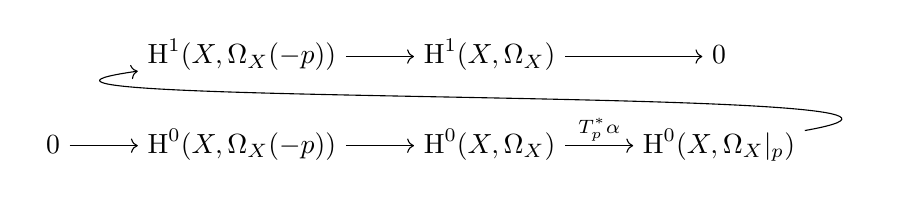
\begin{tikzpicture}[descr/.style={fill=white,inner sep=1.5pt}]
        \matrix (m) [
            matrix of math nodes,
            row sep=1.8em,
            column sep=2.5em,
            text height=1.5ex, text depth=0.25ex
        ]
        {  & \Hnm^1(X, \Omega_X(-p)) &  \Hnm^1(X, \Omega_X) & 0 &  \\
          0  & \Hnm^0(X, \Omega_X(-p)) & \Hnm^0(X, \Omega_X) & \Hnm^0(X, \Omega_X|_p) &  \\
        };

        \path[overlay,->, font=\scriptsize]
        
        (m-1-2) edge (m-1-3)
        (m-1-3) edge (m-1-4)
        (m-2-4) edge[out=10,in=188] (m-1-2)
        (m-2-1) edge (m-2-2)
        (m-2-2) edge (m-2-3)
        (m-2-3) edge node[above, yshift=-2pt] {$T_p^* \alpha$} (m-2-4)
        ;
\end{tikzpicture}
\end{center}
The proposition below follows from standard arguments in homological algebra:

\begin{proposition}\label{prop:dim_of_Albanese_image}
For a general point $p \in X$,
\begin{equation*}
\begin{aligned}
 \dim_{\mathbb{C}} \alpha(X) =\;& \rank T_p^* \alpha  \\ 
 =\;& n-h^0(X, \Omega_X(-p))  \\ 
 =\;& h^1(X, \Omega_X(-p))-h^1(X, \Omega_X).  \\ 
\end{aligned}
\end{equation*}
In particular,
\begin{equation*}
\begin{aligned}
  & \alpha \text{ is surjective} & \Longleftrightarrow\quad& h^0(X, \Omega_X(-p))=0 \\ 
  & \alpha \text{ is finite onto image} & \Longleftrightarrow\quad& h^0(X, \Omega_X(-p))=n-r \\ 
  & \alpha \text{ is constant} & \Longleftrightarrow\quad& h^0(X, \Omega_X(-p))=n \\ 
  & & \Longleftrightarrow\quad& h^1(X, \Omega_X(-p))=h^1(X, \Omega_X) \\ 
  & & \Longleftrightarrow\quad& n=0. \\ 
\end{aligned}
\end{equation*}
\end{proposition}
We will concentrate on the case where $\alpha$ is finite onto its image.\footnote{The general method remains valid in the broader setting, but the Gauss map then takes values in a different space.} Under this assumption, we set $Z = X$ and $A = \Alb(Z)$. The corresponding Gauss map is then a rational map:
% https://q.uiver.app/#q=WzAsNixbMCwwLCJcXHBoaV9aOiJdLFsyLDAsIlxcR3IocixUXjBBKSJdLFsxLDAsIloiXSxbMywwLCJcXEdyKG4tcixcXEhubV4wKFgsXFxPbWVnYV9YKSkiXSxbMywxLCJcXEhubV4wKFgsXFxPbWVnYV9YKC1wKSkiXSxbMSwxLCJwIl0sWzUsNCwiIiwwLHsic3R5bGUiOnsidGFpbCI6eyJuYW1lIjoibWFwcyB0byJ9fX1dLFsyLDEsIiIsMCx7InN0eWxlIjp7ImJvZHkiOnsibmFtZSI6ImRhc2hlZCJ9fX1dLFsxLDMsIlxcY29uZyIsMSx7InN0eWxlIjp7ImJvZHkiOnsibmFtZSI6Im5vbmUifSwiaGVhZCI6eyJuYW1lIjoibm9uZSJ9fX1dXQ==
\[\begin{tikzcd}[row sep={-1mm}]
	{\phi_Z:} &[-10mm] Z &[5mm] {\Gr(r,T^0A)} & [-7mm] {\Gr(n-r,\Hnm^0(X,\Omega_X))} \\
	& p && {\Hnm^0(X,\Omega_X(-p))}
	\arrow[dashed, from=1-2, to=1-3]
	\arrow["\cong"{description}, draw=none, from=1-3, to=1-4]
	\arrow[maps to, from=2-2, to=2-4]
\end{tikzcd}\]
and we have the isomorphisms 
\begin{equation*}
\begin{aligned}
   \mathbb{P}T^{*}_{0}A \cong\;& \mathbb{P}\Hnm^0(X,\Omega_X), \\ 
    \mathbb{P}\Lambda_{Z}=\;& \left\{\, (p,[\omega])  \in Z \times \mathbb{P}T^{*}_{0}A \;\middle|\; \omega(p)=0 \,\right\}  \\ 
    \cong\;& \left\{\,\rule{0mm}{3.2mm} (p,[\omega])  \in Z \times \mathbb{P}T^{*}_{0}A \;\middle|\; \omega \in \Hnm^0(X,\Omega_X(-p)) \,\right\}  \\ 
    \cong\;& \left(\phi_Z, \Id \right)^{-1} I_{n-r, 1},  \\ 
\end{aligned}
\end{equation*}
where 
$$I_{n-r, 1}:= \left\{\, \rule{0mm}{3.2mm} (V,[\omega])  \in \Gr(n-r,n) \times \Gr(1, n) \;\middle|\; \omega \in V \,\right\}$$ 
is the incidence variety relating $\Gr(n-r,n)$ and $\Gr(1, n)$. In that case, 
\begin{equation*}
\begin{aligned}
    \gamma_Z^{-1}([\omega])=\;& \left\{\, p  \in X  \;\middle|\; \omega(p)=0 \,\right\}  \\  
\end{aligned}
\end{equation*}
is the zero set of section $\omega \in \Hnm^0(X,\Omega_X)$. The number $(-1)^r \deg \gamma_Z$ is the index in the Poincaré--Hopf index formula, and the monodromy group $\Gal(\gamma_Z)$ serves as a more refined invariant, encoding subtler aspects of the geometry.

\begin{remark}
One can define the monodromy group in the real (or topological) setting in an analogous manner. Consider the set
$$U:=\left\{\,\omega \in \Gamma(\Omega_M)      \;\middle|\; \rule{0mm}{3.0mm}  \text{ the zeros of $\omega$ are isolated with local index $1$ }  \right\}.$$
A closed loop in $U$ induces a permutation of the zeros of $\omega$, and the monodromy group is defined as the group of all such permutations.

However, when $\dim_{\mathbb{C}} M > 1$, the corresponding monodromy group is always the full symmetric group (as all transpositions occur). As a result, it does not yield any further insight into the topology of the manifold.
\end{remark}

The next proposition shows when the Gauss map $\phi_Z$ is not generic injective.
\begin{proposition}
When $\alpha$ is finite onto its image,
\begin{equation*}
\begin{aligned}
  \;&  \phi_Z \text{ is not generic injective} \\ 
  \Longleftrightarrow\;\;& \text{For general $p \in X$, exists $q \neq p$ such that $h^0(X,\Omega_X(-p-q))=n-r$} \\ 
  \stackrel{\textcolor{purple}{\textbf{?}\footnotemark}}{\Longleftrightarrow}\;\;& \text{For general $p \in X$, exists $S \in X^{[2]}$ such that $p\in S$ and $h^0(X,\Omega_X \otimes \mathcal{I}_S)=n-r$} \\ 
  \Longleftrightarrow\;\;& \text{For all $p \in X$, exists $S \in X^{[2]}$ such that $p\in S$ and $h^0(X,\Omega_X \otimes \mathcal{I}_S)\geqslant  n-r$.} \\ 
\end{aligned}
\end{equation*}
\end{proposition}
\footnotetext{When $n = r$, the map $\varphi_Z$ has a point as its target, so the equivalence is trivial.
When $n > r$, the implication ``$\Rightarrow$" is immediate. For the converse ``$\Leftarrow$", it suffices to show that the image of 
$$\left\{ S \in X^{[2]} \;\middle|\; h^0(X,\Omega_X \otimes \mathcal{I}_S)=n-r   \right\}$$
 under the map $\pi_X:X^{[2]} \longrightarrow X^{(2)} $ does not include the diagonal. Indeed, we can choose a section $s \in \Hnm^0(X,\Omega_X)$ that cuts out finitely many reduced points $p_1,\ldots,p_d$ in $X$. (Well this maybe not so true, since $\phi_Z$ is not always regular, such a section $s$ may vanish along some indeterminacy locus. However, for a general $s$, there will always be at least one isolated zero $p_1$, which is sufficient for our purposes.)
Then for any $S \in \pi_X^{-1}(p_1)$, we have 
$$\Hnm^0(X,\Omega_X \otimes \mathcal{I}_S)  \subsetneqq \Hnm^0(X,\Omega_X(-p_1)).$$
}
This last step relies on the following lemma, combined with the closedness of the tautological correspondence in $X \times X^{[2]}$.
\begin{lemma}
Let $m \in \mathbb{Z}_{>0}$. The function $$h^{\Omega}: X^{[m]} \longrightarrow \mathbb{Z}_{\geqslant 0} \qquad
 S \longmapsto h^0(X,\Omega_X \otimes \mathcal{I}_S)$$ 
is Zariski upper semicontinuous.
\end{lemma}
\begin{proofsketch}
Consider the coherent sheaf $\mathcal{F} \in \Coh(X^{[m]} \times X)$ characterized by the property
$$\mathcal{F}|_{\{S\} \times X} \cong \Omega_X \otimes \mathcal{I}_S,$$
The proposition then follows directly from the semicontinuity theorem \cite[28.1.1]{vakil2017rising}.
\end{proofsketch}

The stratification of $X^{[m]}$ by $h^{\Omega}$ offers a natural generalization of Brill--Noether theory beyond the setting of curves.

At the end of this subsection, let us turn to the setting of a general abelian variety $A$ and a smooth subvariety $\iota_Z: Z \hookrightarrow A$, where $n = \dim_{\mathbb{C}} A$ and $r = \dim_{\mathbb{C}} Z$. Observe that $\iota_Z$ factors through the Albanese variety of $Z$:
% https://q.uiver.app/#q=WzAsMyxbMCwwLCJcXGlvdGFfWjogWiAgIl0sWzEsMCwiXFxBbGIoWikiXSxbMiwwLCJBIl0sWzAsMSwiXFxhbHBoYV9aIl0sWzEsMiwiXFxwaSJdXQ==
\[\begin{tikzcd}[column sep=large]
	{\iota_Z: Z  } & {\Alb(Z)} & A
	\arrow["{\alpha_Z}", from=1-1, to=1-2]
	\arrow["\pi", from=1-2, to=1-3]
\end{tikzcd}\]

We shall also assume that $Z$ generates $A$; it then follows that the map $\pi$ is surjective. The cotangent map of $\iota_Z$ at a point $p \in Z$ factors through $\Hnm^0(Z, \Omega_Z)$:
% https://q.uiver.app/#q=WzAsMyxbMCwwLCJUX3BeKiBcXGlvdGFfWjogVF9wXipBICAiXSxbMSwwLCJcXEhubV4wKFosIFxcT21lZ2FfWikiXSxbMiwwLCJUX3BeKloiXSxbMCwxLCIiLDAseyJzdHlsZSI6eyJ0YWlsIjp7Im5hbWUiOiJob29rIiwic2lkZSI6InRvcCJ9fX1dLFsxLDJdXQ==
\[\begin{tikzcd}[column sep=large]
	{T_p^* \iota_Z: T_p^*A  } & {\Hnm^0(Z, \Omega_Z)} & {T_p^*Z}
	\arrow[hook, from=1-1, to=1-2]
	\arrow[from=1-2, to=1-3]
\end{tikzcd}\]
For convenience, abbreviate $V := T_0^*A \cong T_p^*A$, and view $V$ as a subspace of $\Hnm^0(Z, \Omega_Z)$.
\begin{proposition}
Assume that $Z$ is embedded in $A$ and generates $A$, and let $V := T_0^*A$. Then
$$\dim_{\mathbb{C}} \Hnm^0(Z,\Omega_Z(-p)) \cap V =n-r \qquad \text{ for all $p \in Z$}$$
It follows that the Gauss map is a regular morphism
\[\begin{tikzcd}[row sep={-1mm}]
	{\phi_Z:} &[-10mm] Z &[5mm] {\Gr(r,T^0A)} & [-7mm] {\Gr(n-r,V)} \\
	& p && {\Hnm^0(Z,\Omega_Z(-p)) \cap V}
	\arrow[from=1-2, to=1-3]
	\arrow["\cong"{description}, draw=none, from=1-3, to=1-4]
	\arrow[maps to, from=2-2, to=2-4]
\end{tikzcd}\]
 Furthermore, 
\begin{equation*}
\begin{aligned}
  \;&  \phi_Z \text{ is not generic injective} \\ 
  \Longleftrightarrow\;\;& \text{For general $p \in X$, exists $q \neq p$ such that $h^0(X,\Omega_X(-p-q)) \cap V =n-r$} \\ 
  \Longleftrightarrow\;\;& \text{For all $p \in X$, exists $S \in X^{[2]}$ such that $p\in S$ and $h^0(X,\Omega_X \otimes \mathcal{I}_S) \cap V=n-r$.} \\ 
\end{aligned}
\end{equation*}
\end{proposition}

\begin{ques}
For an $r$-dimensional smooth variety $Z$ whose Albanese map $\alpha_Z$ is an embedding, which subspaces $V \subset \Hnm^0(Z, \Omega_Z)$ can arise as the cotangent space of some abelian quotient variety of $\Alb(Z)$?
\end{ques}

The precise formulation of this question is somewhat ambiguous, and depending on the interpretation, it may turn out to be either relatively straightforward or extremely difficult. On the one hand, the classification of abelian subvarieties of $A$ via symmetric idempotents in $\End_{\mathbb{Q}}(A)$ is well established \cite[Theorem 5.3.2]{BL04}. On the other hand, explicitly computing $\End_{\mathbb{Q}}(A)$ can be highly nontrivial when $A$ is a non-simple Albanese variety—even in the case where $A$ arises from a curve.

 

\section{Families of subvarieties}

In this section, we move from the study of monodromy groups to a more direct analysis of the subvarieties themselves. Given an initial subvariety, one can naturally generate a family of subvarieties. Our goal here is to define these families and investigate their properties.

\begin{proposition}
All irreducible conic Lagrangian cycles in $T^*A$ are of the form $\Lambda_Z$ for some irreducible subvariety $Z \subset A$. This yields a one-to-one correspondence between irreducible conic Lagrangian cycles in $T^*A$ and irreducible subvarieties of $A$:
$$\left\{\text{ irreducible conic Lagrangian cycles in $T^*A$ }   \right\} \longleftrightarrow \left\{\text{ irreducible subvarieties in $A$ }   \right\}$$
\end{proposition}

\begin{proofsketch}
For any irreducible conic Lagrangian cycle $\mathbf{\Lambda} \subset T^*A$, let $Z$ denote the image of $\mathbf{\Lambda}$ under the natural projection $T^*A \to A$. Our goal is to show that $\mathbf{\Lambda} = \Lambda_Z$.
\begin{itemize}
\item By definition, $\mathbf{\Lambda} \subset T^*A|_Z$.
\item Since $\mathbf{\Lambda}$ is conic, we have $s(Z) \subset \mathbf{\Lambda}$, where $s : A \to T^*A$ denotes the zero section.
\item Since $\mathbf{\Lambda}$ is Lagrangian and $s(Z) \subset \mathbf{\Lambda}$, we have $\mathbf{\Lambda} \subset \Lambda_Z$.
\item Since $\Lambda_Z$ is irreducible with $\dim_{\mathbb{C}} \mathbf{\Lambda} = \dim_{\mathbb{C}} \Lambda_Z = n$, we have $\mathbf{\Lambda} = \Lambda_Z$.
\end{itemize}
\end{proofsketch}

Why do we shift attention from $Z$ to $\Lambda_Z$ as the main object of study? One reason is the uniformity of $\Lambda_Z$: it always has dimension $n$, and in most cases, the natural map $\Lambda_Z \to T_0^* A$ is generically finite, with fibers lying inside $A$.

\begin{definition}[Clean cycle]
An irreducible Lagrangian cycle $\mathbf{\Lambda} \subset T^*A$ is called clean if the composed projection
$$\mathbf{\Lambda} \longrightarrow T^*A \twoheadrightarrow T_0^*A$$
is generically finite.
\end{definition}

Another important reason is that the space of weighted clean conic Lagrangian cycles naturally acquires a convolution structure, arising from the group law on $A$, which plays a central role in the analysis.

\begin{proposition}
The group of weighted clean conic Lagrangian cycles
\begin{equation*}
\begin{aligned}
  \mathcal{L}(A):=\;& \left\{ \text{weighted clean conic Lagrangian cycles in }T^*A \right\}  \\ 
  =\;& \left\{ \raisebox{1.5mm}{$\displaystyle\sum_{\substack{Z_i \subset A \\ \text{irr clean}}}$}n_i \Lambda_{Z_i}\; \middle|\; n_i \in \mathbb{Z} \right\}  \\ 
\end{aligned}
\end{equation*}
has a natural convolution structure as follows: 
\begin{equation*}
\begin{aligned}
  \Lambda_{Z_1} \circ \Lambda_{Z_2}=\;& \text{ the clean part of }(a,\Id_{T_0^* A})_* \left( \Lambda_{Z_1} \times_{T_0^* A} \Lambda_{Z_2} \right) \\ 
  =\;& \overline{(a,\Id_{U})_* \left( \Lambda_{Z_1}|_U \times_{U} \Lambda_{Z_2}|_U \right)} \\ 
\end{aligned}
\end{equation*}
where 
$$U:=\left\{ \xi \in T_0^*A \; \middle|\; \rule{0mm}{3.4mm}\deg \phi_{Z_i}= \# \phi_{Z_i}^{-1}(\xi) \text{ for } i=1,2 \right\}$$
and $a: A \times A \longrightarrow A$ is the addition map in $A$. The general convolution is defined by $\mathbb{Z}$-linear extension.
\end{proposition}

\begin{proofsketch}
To establish the claim, it suffices to show that $\Lambda_{Z_1} \circ \Lambda_{Z_2}$ defines a weighted conic Lagrangian cycle. The conic property follows directly from the definition, while the Lagrangian condition can be verified at a general point $(p_1 + p_2, \xi) \in \Lambda_{Z_1} \circ \Lambda_{Z_2}$.
\end{proofsketch}

We now consider the projective versions of all objects involved, so that we may make use of properness. To simplify notation, we abbreviate $\mathbb{P}T^{*}_{0}A$ by $\mathbb{P}^{\vee}$.

\begin{lemma}\label{lem:mon_of_prod}\
\begingroup
\upshape
%\setlist{itemsep=-0.4em}
\renewcommand\labelenumi{(\theenumi)}
\begin{enumerate}[(1)]
\item Suppose that $\mathbb{P}\Lambda_{Z_1}, \mathbb{P}\Lambda_{Z_1} \subset \mathbb{P}T^*A$ admit monodromy representations $$\rho_{\gamma_{Z_i}}: \pi_1(U,\xi_0) \longrightarrow \Aut\left(\gamma_{Z_i}^{-1}(\xi_0)\right),$$ 
then $\mathbb{P}\Lambda_{Z_1} \times_{\mathbb{P}^{\vee}} \mathbb{P}\Lambda_{Z_2} \subset A\times A \times \mathbb{P}^{\vee}$ admits monodromy representation given by
$$(\rho_{\gamma_{Z_1}},\rho_{\gamma_{Z_2}}): \pi_1(U,\xi_0) \longrightarrow \Aut\left(\gamma_{Z_1}^{-1}(\xi_0) \times \gamma_{Z_2}^{-1}(\xi_0)\right),$$ 
\item When $Z_1=Z_2=Z$, we obtain an one-to-one correspondence:
$$\left\{ 
\begin{aligned}
  &\text{ irr components of } \mathbb{P}\Lambda_{Z} \times_{\mathbb{P}^{\vee}} \mathbb{P}\Lambda_{Z}  \\ 
  &\hspace{10mm}\text{ with a surjection to } \mathbb{P}^{\vee}
\end{aligned}
 \right\} \longleftrightarrow 
\left\{ 
\begin{aligned}
  &\Gal(\gamma_{Z})\text{-orbits of }  \\ 
  &\;\;\gamma_{Z}^{-1}(\xi_0) \times \gamma_{Z}^{-1}(\xi_0)
\end{aligned}
 \right\} 
 $$
\end{enumerate}
\endgroup
\end{lemma}
\begin{proofsketch}
Statement (1) holds by definition. The proof of (2) reduces to the following purely topological statement:
\begin{claim}
Let $\pi: E \longrightarrow B$ be a (unramified) covering space over a manifold $B$ with deck transformation group $G$, then
$$\left\{ \rule{0mm}{3.1mm}\text{ connected components of }E \times_B E \;\right\} \longleftrightarrow \left\{   \;G\text{-orbits of } \pi^{-1}(b_0) \times \pi^{-1}(b_0)\; \right\}. $$
\end{claim}
\noindent The claim follows directly from the correspondence between covering spaces over $B$ and $\pi_1(B)$-sets; see \cite[Theorem 1.38]{Ha02}.
\end{proofsketch}

Generalizing the argument of Lemma \ref{lem:mon_of_prod}, we arrive at the following lemma.

\begin{lemma}
For $d=\deg \gamma_{Z}$, $\xi_0 \in T_0^* A$ a general point, write
\begin{equation*}
\begin{aligned}
  \mathbb{P}\Lambda_{Z}^{\times d} :=\;&\;\; \mathbb{P}\Lambda_{Z} \times_{\mathbb{P}^{\vee}}\mathbb{P}\Lambda_{Z} \times_{\mathbb{P}^{\vee}} \cdots \times_{\mathbb{P}^{\vee}} \mathbb{P}\Lambda_{Z} && \subset A^d \times \mathbb{P}^{\vee}\\ 
  \gamma_{Z}^{-1}(\xi_0)^{d} :=\;& \gamma_{Z}^{-1}(\xi_0) \times \gamma_{Z}^{-1}(\xi_0) \times \cdots \times \gamma_{Z}^{-1}(\xi_0) && \subset A^d \\ 
\end{aligned}
\end{equation*}
\begingroup
\upshape
%\setlist{itemsep=-0.4em}
\renewcommand\labelenumi{(\theenumi)}
\begin{enumerate}[(1)]
\item we obtain an one-to-one correspondence:
$$\left\{ 
\begin{aligned}
  &\text{ irr components of } \mathbb{P}\Lambda_{Z}^{\times d}  \\ 
  &\hspace{0mm}\text{ with a surjection to } \mathbb{P}^{\vee}
\end{aligned}
 \right\} \longleftrightarrow 
\left\{ 
\begin{aligned}
  &\Gal(\gamma_{Z})\text{-orbits of }  \\ 
  &\hspace{8mm}\gamma_{Z}^{-1}(\xi_0) ^d
\end{aligned}
 \right\} 
 $$
\item Write
\begin{equation*}
\begin{aligned}
  \Delta_d :=\;&\left\{ (p_1,\ldots,p_d) \in A^d \;\middle|\; p_i=p_j \text{ for some } i \neq j  \right\} && \subset A^d \\ 
  \mathbb{P}\Lambda_{Z}^{[d]} :=\;& \overline{\left( \mathbb{P}\Lambda_{Z}^{\times d} \smallsetminus \left( \Delta_d \times \mathbb{P}^{\vee} \right) \right)|_U} && \subset A^d \times \mathbb{P}^{\vee}\\ 
\end{aligned}
\end{equation*}
Fix a general point $\xi_0 \in \mathbb{P}^{\vee}$ and a well-order for $\gamma_{Z}^{-1}(\xi_0)$, one can identify $S_d \cong \gamma_{Z}^{-1}(\xi_0)^d \smallsetminus \Delta_d$, and 
$$\left\{ 
\text{ irr components of } \mathbb{P}\Lambda_{Z}^{[d]}  
 \;\right\} \longleftrightarrow 
\left\{ \;\rule{0mm}{3.3mm}
\Gal(\gamma_{Z})\text{-orbits of }  S_d
 \;\right\} 
 $$
 In reference, $\Delta_d$ is usually called the big diagonal.
\end{enumerate}
\endgroup
\end{lemma}

From this point on, we fix an irreducible component of $\mathbb{P}\Lambda_{Z}^{[d]}$, denoted by $\mathbb{P}\Lambda_{Z}^{\univ}$. As we will see in Definition A, this variety generates all subvarieties within the families under consideration.

\begin{definition}[The subvariety $Z^{(m)}$]
For any tuple $(m) = (m_1, \ldots, m_d) \in \mathbb{Z}^d$, we define the weighted sum map
$$a^{(m)}: A^d \longrightarrow A \qquad (p_1,\ldots,p_d) \longmapsto \sum_{i=1}^{d} m_ip_i.$$
We also define 
$$\mathbb{P}\Lambda_{Z}^{(m)}: = \left( a^{(m)},\Id_{\mathbb{P}^{\vee}}  \right)_* \mathbb{P}\Lambda_{Z}^{\univ}.$$
as the (projectivized) weighted Lagrangian cycle in $\mathbb{P}T^*A$. The projective cycle $\mathbb{P}\Lambda_{Z}^{(m)}$ is irreducible but may appear with multiplicities. We can therefore write
$$\mathbb{P}\Lambda_{Z}^{(m)} = c_Z^{(m)}  \mathbb{P}\Lambda_{Z^{(m)}}$$
where $c_Z^{(m)} \in \mathbb{Z}_{>0}$ and $Z^{(m)} \subset A$ are uniquely determined. This gives rise to a family of subvarieties parametrized by $\mathbb{Z}^d$.
\end{definition}

The next lemma gathers some basic properties of $Z^{(m)}$. Observe that $S_d=\Aut\left(\gamma_{Z}^{-1}(\xi_0)\right)$ acts naturally on $\mathbb{Z}^d$ via
$$g(m)=\left(m_{g(1)},\ldots , m_{g(d)}\right) \in \mathbb{Z}^d.$$

\begin{lemma}\
\begingroup
\upshape
%\setlist{itemsep=-0.4em}
\renewcommand\labelenumi{(\theenumi)}
\begin{enumerate}[(1)]
\item For all $g\in \Gal(\gamma_{Z})$, we have $ Z^{g(m)}=Z^{(m)}$, $c_Z^{g(m)}=c_Z^{(m)}$;
\item For $(m)=(1,0,\ldots,0)\in \mathbb{Z}^d$, $Z^{(m)}=Z$;
\item For all $(m), (m') \in \mathbb{Z}^d$, we have  $\mathbb{P}\Lambda_{Z}^{(m)} \circ \mathbb{P}\Lambda_{Z}^{(m')} \supseteq \mathbb{P}\Lambda_{Z}^{(m+m')}$;
\item The group $\left< \mathbb{P}\Lambda_{Z^{(m)}} \right>_{\Abel}$ is closed under the convolution product.
\end{enumerate}
\endgroup
\end{lemma}

\begin{ques}\label{ques:homo_class_of_subvarieties}
Can we compute the dimension and the homology class for these subvarieties $Z^{(m)}$?
\end{ques}

At first glance, this question may appear naive, but it turns out to be extremely challenging. The main difficulty lies in determining the homology class of $\mathbb{P}\Lambda_{Z}^{\univ}$. Once this is known, one can compute the pushforward to obtain the homology class of $\mathbb{P}\Lambda_{Z}^{(m)}$, from which both $\dim_{\mathbb{C}} Z^{(m)}$ and the homology class of $Z^{(m)}$ (up to a scalar factor $c_Z^{(m)}$) can be extracted.

However, standard intersection theory yields only the homology class of $\mathbb{P}\Lambda_Z^{[d]}$, via the Chern–Mather class of $Z$. At present, there is no known method for computing the homology class of a single irreducible component of $\mathbb{P}\Lambda_Z^{[d]}$. Although we can distinguish these components topologically, we lack tools to compute their topological invariants, which presents an unfortunate limitation.

Nevertheless, Question \ref{ques:homo_class_of_subvarieties} can still be addressed in certain special situations. For instance, when $\Gal(\gamma_Z) = S_n$, the space $\mathbb{P} \Lambda_Z^{[d]}$ is known to be irreducible, enabling explicit computation. Similarly, when $Z = -Z$ and $\Gal(\gamma_Z) = W(C_{d/2})$, one can impose additional conditions (e.g., $p_{2l-1} = -p_{2l}$) to guarantee the uniqueness of $\mathbb{P} \Lambda_Z^{\univ}$, which again allows us to perform the computation.

\begin{ques}
Suppose $d = 2d_0$ with $d_0$ even, $(m) \in \mathbb{Z}^d$, and $g \in W(C_{d/2}) \smallsetminus W(D_{d/2})$. Is it possible to construct an example with $Z = -Z$ and $\Gal(\gamma_Z) = W(D_{d/2})$, yet $\dim_{\mathbb{C}} Z^{g(m)} \neq \dim_{\mathbb{C}} Z^{(m)}$?
\end{ques}

\begin{ques}
Suppose that $Z$ is the Fano surface of a smooth cubic threefold, and let $A := \Alb(Z)$. How can we compute the homology class of $Z^{(m)}$?
\end{ques}


\section{Tannakian formalism}


For simplicity, we work over the base field $\kappa = \mathbb{C}$. Let $A$ denote a fixed complex abelian variety, and let $\Perv(A)$ denote the category of perverse sheaves on $A$ with coefficients in $\mathbb{Q}$. For any algebraic group $G$, we denote by $\Rep(G)$ the category of algebraic representations of $G$.

Following the approach of \cite{KW15vanishing}, we work in the quotient category $\overline{\Perv}(A) = \Perv(A) / N(A)$, where $N(A) \subset \Perv(A)$ is the Serre subcategory of negligible complexes. A complex $\mathcal{F}$ is defined to be negligible if $\chi(A, \mathcal{F}) = 0$. This quotient category admits a natural convolution structure, and every finitely generated tensor subcategory of it is Tannakian, with a reductive Tannaka group $G$ (see \cite[Thm 7.1 \& Cor 9.2]{KW15vanishing}). In particular, for any perverse sheaf $\delta \in \overline{\Perv}(A)$, the full subcategory generated by $\delta$ is categorically equivalent to the representation category of an algebraic group $G$:
$$\left< \delta, * \right> \cong \Rep(G).$$


%\nocite{Eberhardt2022Koszul}	% cite articles which are not cited in the document yet

% Remember to protect the uppercase of people's name and LaTeX symbols

\bibliographystyle{plain}
\bibliography{reference}
\end{document}